\appendix
\chapter{Appendix: Tomographic Analysis of BOSS DR12 galaxies}
\section{Correspondence between overdensity and number counts Pseudo-$C_{\ell}$ estimators}\label{Apx:PCL}
In Section \ref{Sec:Measurements}, I showed the Pseudo-$C_{\ell}$ estimator for galaxy overdensity maps. To link this with what is most commonly done in the literature, one can show that this galaxy overdensity measure is closely related to the more familiar galaxy number counts estimator as seen in \cite{Peebles1973,ScharfLahav1992,FisherLahav1994,Blake2007,Thomas2011}. For the purpose of this section, I define the galaxy overdensity quantities with an upper $\delta$ index and the number counts quantities with a $n$ upper index. Example: the galaxy overdensity angular power spectra is represented by $C^{\delta}_{\ell}$.

\qquad I start the derivation by multiplying the overdensity spherical harmonics coefficients from Equation \eqref{Eq:AlmPix} by $\bar n^g_i  = n^g_{tot,i}/\Delta \Omega_{tot}$. Equation \eqref{Eq:D_lm_ij} then becomes:

\begin{align}
\label{doesnt_look_helpful_but_is}
{\bar n^g_i \bar n^g_j} D^{\delta, ij}_{\ell m} \approx & \left[ \sum_p^{N_{pix}} \delta_{p,i}^g \Delta\Omega_p \bar n^g_i Y_{\ell m}^{\ast}(\theta_p,\phi_p) \right]\left[ \sum_p^{N_{pix}} \delta_{p,j}^g \Delta\Omega_p \bar n^g_j Y_{\ell m}^{\ast}(\theta_p,\phi_p) \right]
\end{align}
where I bear in mind that different subsamples $ i $ and $j$ can have different total numbers of galaxies and different galaxies in each pixel, but use the same pixels. 

\qquad Using Equation \eqref{Eq:define_delta_p} one can write
\EQ{}{
\delta_p^g \Delta\Omega_p \bar n^g = n_p^g - \Delta\Omega_p \bar n^g.
}

\noindent Now, we can use the above expression to rewrite Equation \ref{doesnt_look_helpful_but_is} as:

\begin{align}
{\bar n^g_i \bar n^g_j} D^{\delta, ij}_{\ell m} & \approx  \left[ \sum_p^{N_{pix}} \left( n_{p,i}^g - \bar n^g_i \Delta\Omega_p \right) Y_{\ell m}^{\ast}(\theta_p,\phi_p) \right] \left[ \sum_p^{N_{pix}}  \left( n_{p,j}^g - \bar n^g_j \Delta\Omega_p \right) Y_{\ell m}^{\ast}(\theta_p,\phi_p) \right] .
\end{align}

\qquad Analysing just the individual terms on the square brakes in the above equation, one has

\EQ{}{
\sum_p^{N_{pix}} Y_{\ell m}(\theta_p,\phi_p)\Delta\Omega_p \approx \int Y_{\ell m}^{\ast}(\theta,\phi) d\Omega \equiv I_{\ell m}
}
where I can therefore see that this term is approximately equivalent to the shot noise correction term $I_{\ell m}$ from \cite{Blake2007,Thomas2011}. The second term can also be re-expressed as:

\begin{align}
\sum_p^{N_{pix}} Y_{\ell m}(\theta_p,\phi_p) n_p^g &\approx \sum_{g^\prime} Y_{\ell m}(\theta_{g^\prime},\phi_{g^\prime}) \\ \nonumber
								&= \sum_{g^\prime} \int \delta_D(x_{g^\prime}-x) Y_{\ell m}(\theta,\phi) d\Omega
\end{align}
\noindent where the index $g^\prime$ runs over galaxies in the sample that have not been excluded by the mask and $\delta_D(x)$ is the Dirac delta function. I can reverse the order of summation and integration, and express the number count function as:
\EQ{}{
\sigma_1 = \sum_{g^\prime} \delta(x_{g^\prime}-x),
} 

\noindent i.e., the galaxy distribution is a sum of delta functions at the locations of the galaxies, and hence the integral over this function is the total number of galaxies in that area. The function $\sigma_1$ is the filtered galaxy distribution, which has been masked. It is related to the full galaxy distribution $\sigma_0$ by:
\EQ{}{
\sigma_1(\theta,\phi) = \sigma_0(\theta,\phi) W(\theta,\phi),
}

\noindent where $W: S^2 \rightarrow \mathbb{B}$ is a binary filter, and:

\EQ{}{
\sigma_0 = \sum_g \delta(x_g - x)
}

\noindent runs over the full underlying set of galaxies.

\qquad One can therefore write:
\begin{align}
\sum_p^{N_{pix}} Y_{\ell m}(\theta_p,\phi_p)n_p^g  & \approx \int \sigma_0(\theta,\phi)W(\theta,\phi)Y_{\ell m}(\theta,\phi)d\Omega \\ & = a_{\ell m}
\end{align}
\noindent where $a_{\ell m}$ are the spherical harmonic coefficients of the filtered galaxy number count field. Finally, one ends up with 
\begin{align}
\bar n^g_i \bar n^g_j D^{\delta, ij}_{\ell m} & \approx  \frac{\left[ a_{\ell m}^i - \bar n_i^g I_{\ell m} \right] \left[ a_{\ell m}^j - \bar n_j^g I_{\ell m} \right]}{J_{\ell m}} \\ & = D^{n,ij}_{\ell m},
\end{align}
in other words, the overdensity and number count power spectra differ only by a factor of the number density of galaxies in each tomographic bin involved.


\section{Code comparison}\label{Apx:Code_Comparison}
The results presented in Chapter \ref{Chap:BOSS} used \class \citep{Class} (background evolution and perturbations) and the $C_{\ell}$ estimation code \uclcl (projected statistics). Here, I show a comparison for $C_{\ell}$s calculated with both \class (integrated functionality from the former \texttt{CLASSGAL} code \citep{CLASSgal}) and \texttt{CAMBSources} \citep{CambSources}, matching cosmologies as closely as possible. I also show the derivatives calculated with respect to key cosmological parameters. In this comparison I use Gaussian redshift bins, since this is the functionality provided in \class and \texttt{CAMBSources}. Two redshift bins are chosen with $\bar{z} = \{0.5,0.6\}$ and $\sigma_z = 0.05$ to be of comparable size to the redshift bins used in the body of the chapter; auto and cross-correlations are calculated. Codes are run with their default accuracy parameters. 

\subsection{Auto- and cross-power spectrum precision}
The auto-power spectrum for a bin with $\bar{z} = 0.5$ and $\sigma_z = 0.05$ is shown in Figure \ref{fig:Auto_Precision}, calculated in each of the three codes for a flat $\Lambda$CDM cosmology with $\Omega_b = 0.05$, $\Omega_{cdm} = 0.25$, $h = 0.67$, $\log(A_s \times 10^{-10}) = 3.2$, $n_s = 0.95$. Codes are in sub-percent level agreement up to $\ell \approx 200$ (although the \class low $\ell$ RSDs disagree to a slightly larger extent), after which there is a small discrepancy between \class and \texttt{CAMBSources} non-linear density perturbations. As one might expect, the differences between \textsc{uclcl} and \texttt{CAMBSources} trace the differences between \class and \texttt{CAMBSources} as the former two share the same perturbations, i.e. $P(k)$.

\begin{figure}
\begin{center}
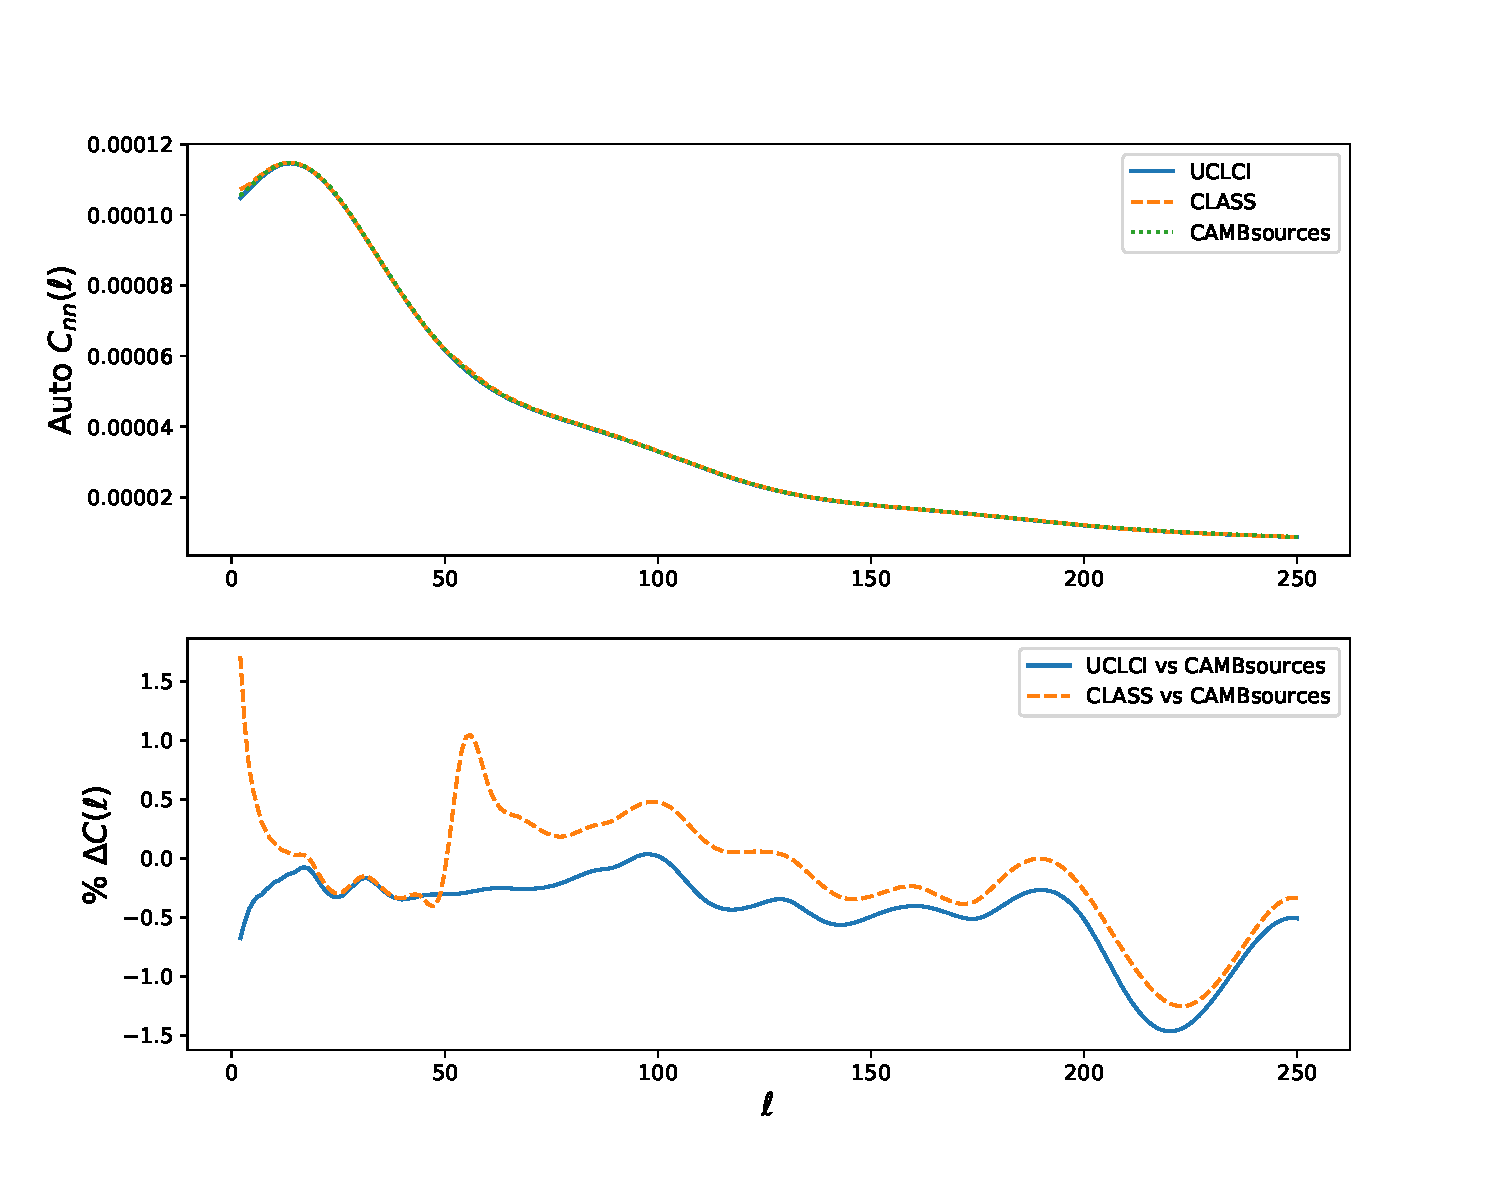
\includegraphics[width=\textwidth]{BOSS-FIGS/PrecAutos.pdf}
\caption[Code comparison between \uclcl, \class, and \texttt{CAMBSources} for the auto-$C_{\ell}$s calculation.]{Auto-correlation $C_{\ell}$ ($\bar z = 0.5, \sigma_z = 0.05$) comparison the three codes \uclcl, \class, and \texttt{CAMBSources}. The upper panel shows the three $C(\ell)$s over-plotted, whilst the lower panel shows the percentage difference between \uclcl / \class compared to \texttt{CAMBSources}: $\frac{C_\camb-C_{\uclcl / \class}}{C_{\camb}}\times 100$.}
\label{fig:Auto_Precision}
\end{center}
\end{figure}

\qquad The same trend is observed in the cross-correlations in Figure \ref{fig:Cross_Precision}, with a notable wobble in the \class cross-correlation presumably when transitioning between approximation schemes (and thus possibly remedied by adjusting accuracy parameters away from the default). 



\subsection{Sensitivity to cosmological parameters} \label{App_accuracy}
\begin{figure}
\begin{center}
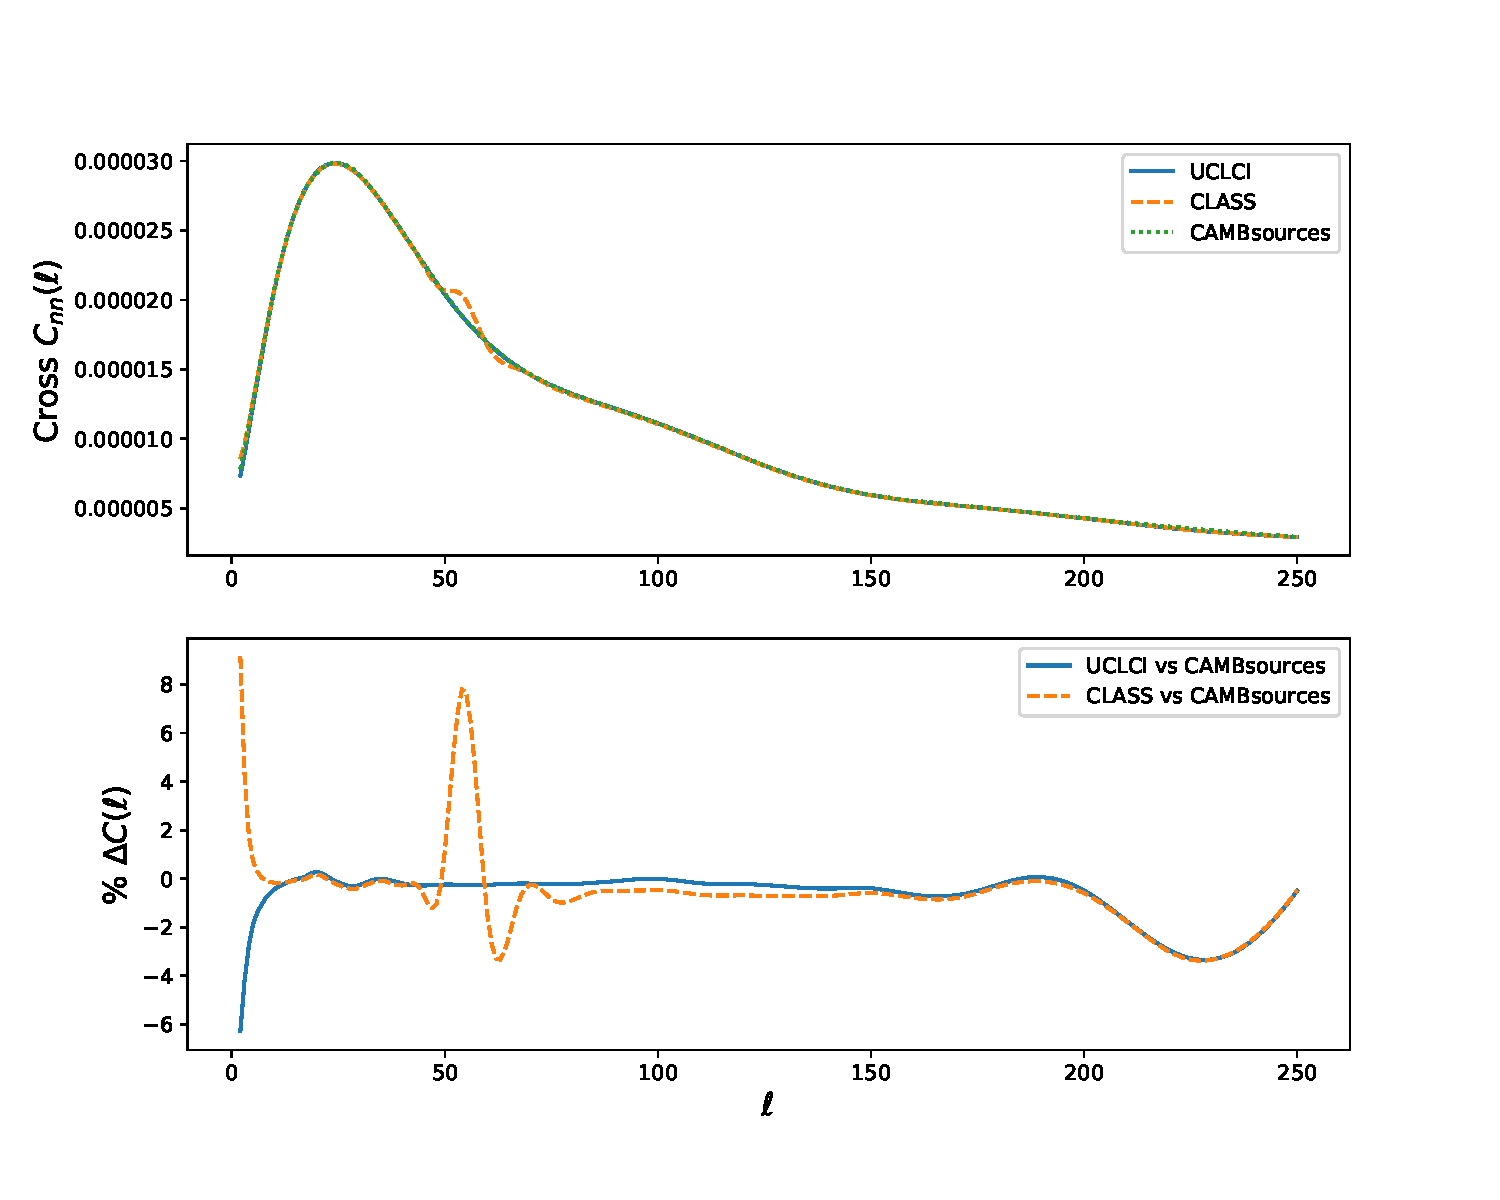
\includegraphics[width=\textwidth]{BOSS-FIGS/PrecCross.pdf}
\caption[Code comparison between \uclcl, \class, and \texttt{CAMBSources} for the cross-$C_{\ell}$s calculation.]{Cross-correlation $C_{\ell}$ ($\bar z^i = 0.5, \bar z^j = 0.6, \sigma_z = 0.05$) comparison the three codes \uclcl, \class, and \texttt{CAMBSources}. The upper panel shows the three $C_{\ell}$s over-plotted, whilst the lower panel shows the percentage difference between \uclcl / \class compared to \texttt{CAMBSources}: $\frac{C_{\camb}-C_{\uclcl / \class}}{C_{\camb}}\times 100$. Again \uclcl follows \class closely, except in the RSDs and in a distinctive wobble around $l \approx 50$ where \class is presumably transitioning between some approximation schemes.}
\label{fig:Cross_Precision}
\end{center}
\end{figure}
In order to check that the accuracy of the codes is not strongly cosmology dependent, the comparison are also made for variations on $h$, and $w_0$ over sensible ranges of the parameters. It is crucial that the sensitivity to the cosmological parameters not be overwhelmed by the (approximately percent level) uncertainty in the $C_{\ell}$ calculation itself. It is also important to check that the derivatives w.r.t. the cosmological parameters are consistent between the codes, as this will ensure the $C_{\ell}$s change consistently as one moves away from the fiducial cosmology.

\qquad In Figure \ref{fig:h_Precision} one can see that the $C_{\ell}$s for $h = 0.64, 0.67, 0.70$ are clearly delineated and their differences significantly larger than the differences between the $C_{\ell}$s from different codes. With $w$ over the range $-1.1$ to $-0.9$, shown in Figure \ref{fig:w_Precision}, one can see that at low $l$ the $C_{\ell}$s are well distinguished from each other, but at high $l$ $w$ has little effect, and thus is unlikely to be distinguished from the uncertainties inherent in the non-linear regime. In Figure \ref{fig:Diff_w} one can also see that the variation at high $l$ is significantly different for \uclcl and \texttt{CAMBSources}, likely originating from the difference in the perturbations between \class and \texttt{CAMBSources}. Nevertheless, the shape of the derivatives w.r.t. to $w$ up to $\ell \approx 200$, and w.r.t. $h$ throughout the $\ell$ range, look consistent with \texttt{CAMBSources}. This shows that the $C_{\ell}$s are changing in the correct way around this fiducial cosmology, and will yield the correct shape of posterior contours. 

\begin{figure}
\begin{center}
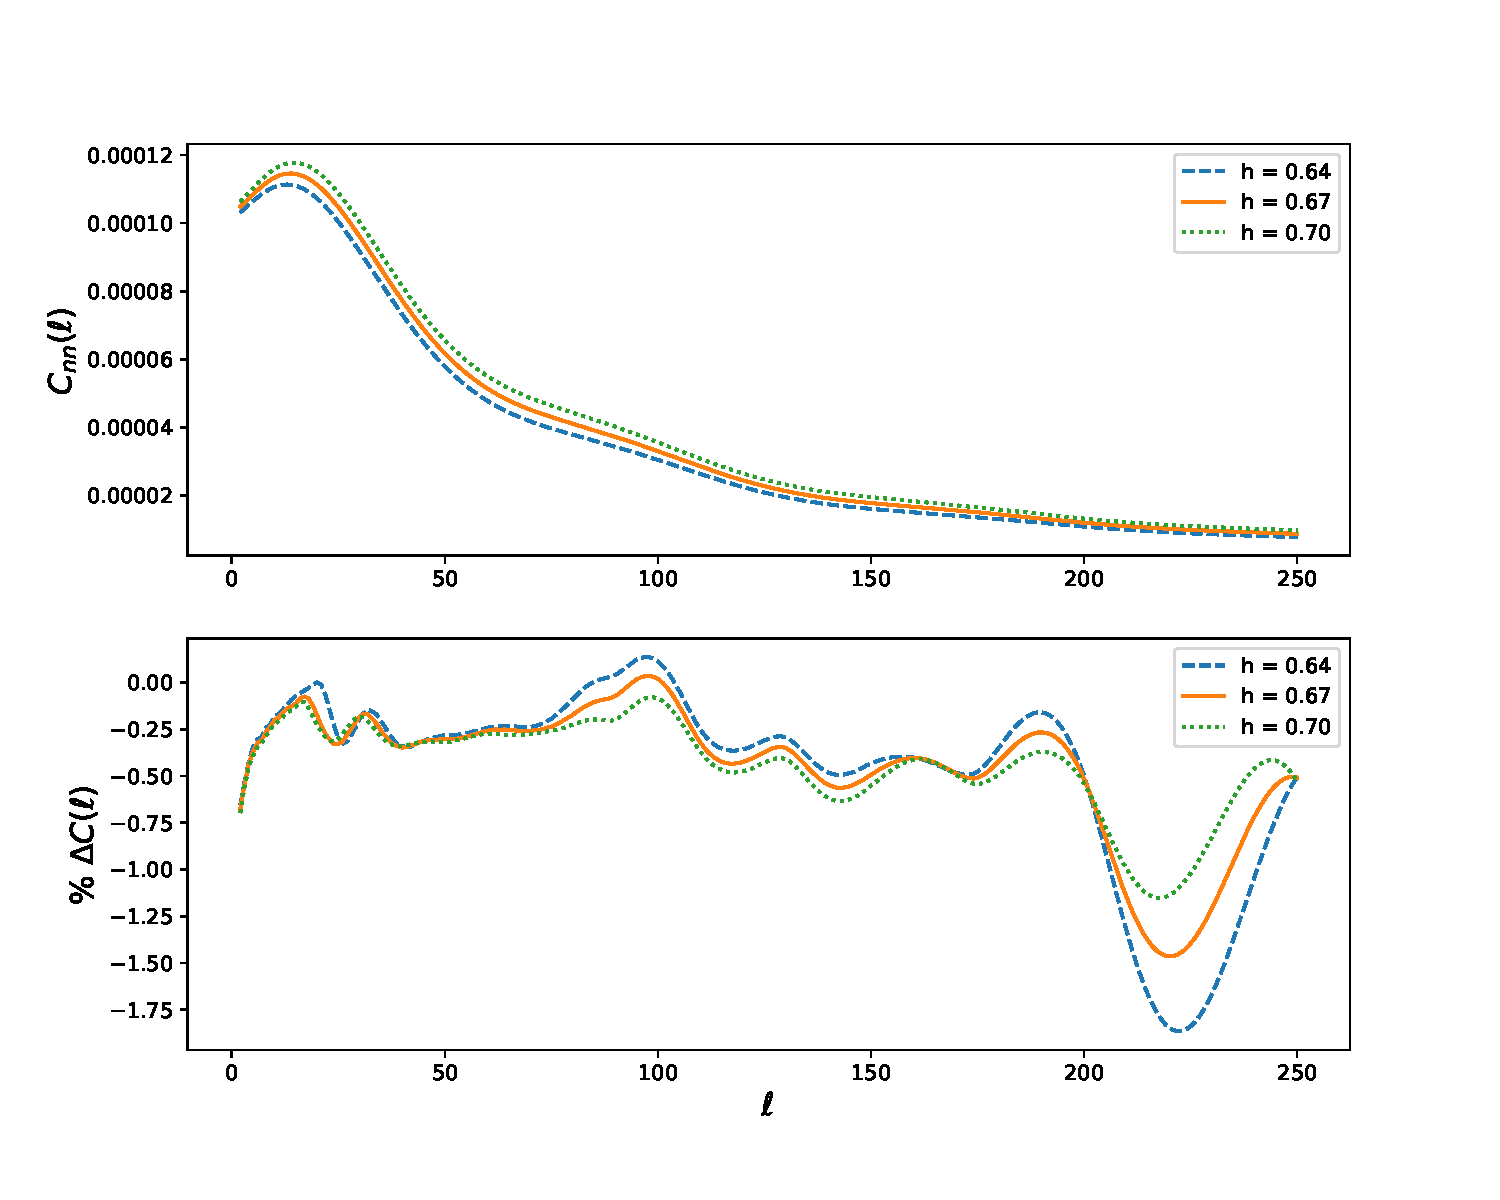
\includegraphics[scale=0.60]{BOSS-FIGS/PrecH.pdf}
\caption[Auto-correlations ($\bar z = 0.5$) for three values of $h$ calculated in \uclcl and comparison between \class and \texttt{CAMBSources}]{The top panel shows the auto-correlations ($\bar z = 0.5$) for three values of $h$ calculated in \uclcl. The lower panel shows the percentage difference of each of these $C_{\ell}$s with the corresponding $C_{\ell}$s from \texttt{CAMBSources} (matching values of $h$).}
\label{fig:h_Precision}
\end{center}
\end{figure}

\begin{figure}
\begin{center}
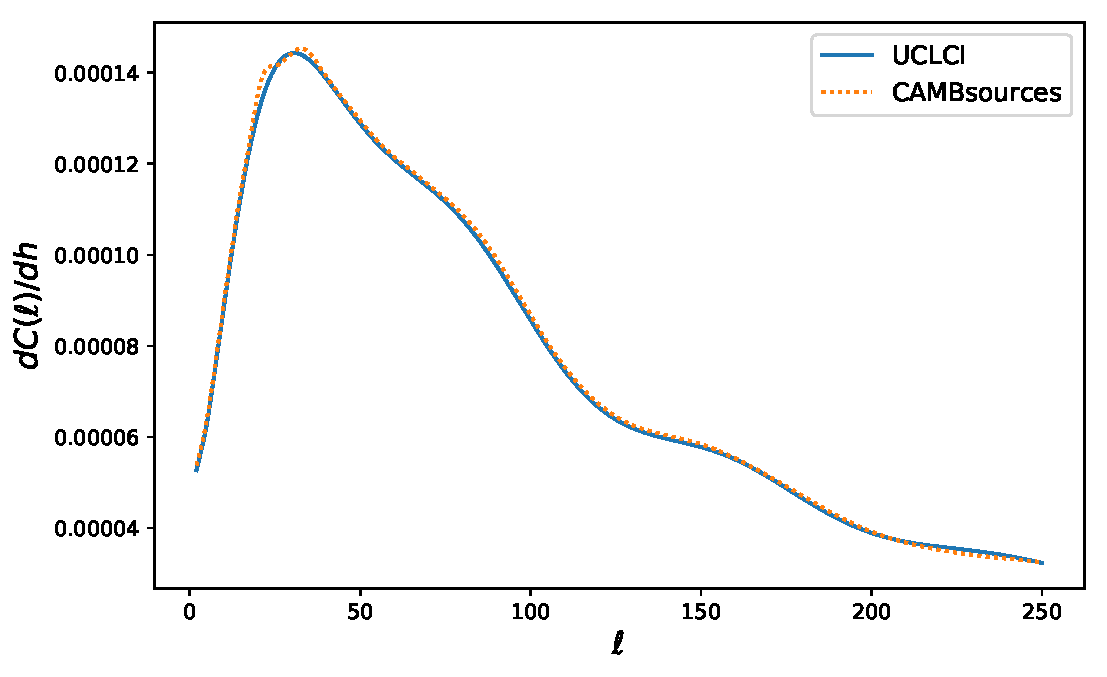
\includegraphics[scale=0.60]{BOSS-FIGS/PrecDh.pdf}
\caption{Comparison of $C_{\ell}$ derivatives $\frac{d C_{\ell}}{dh}$ between \uclcl and \texttt{CAMBSources}.}
\label{fig:Diff_h}
\end{center}
\end{figure}

\begin{figure}
\begin{center}
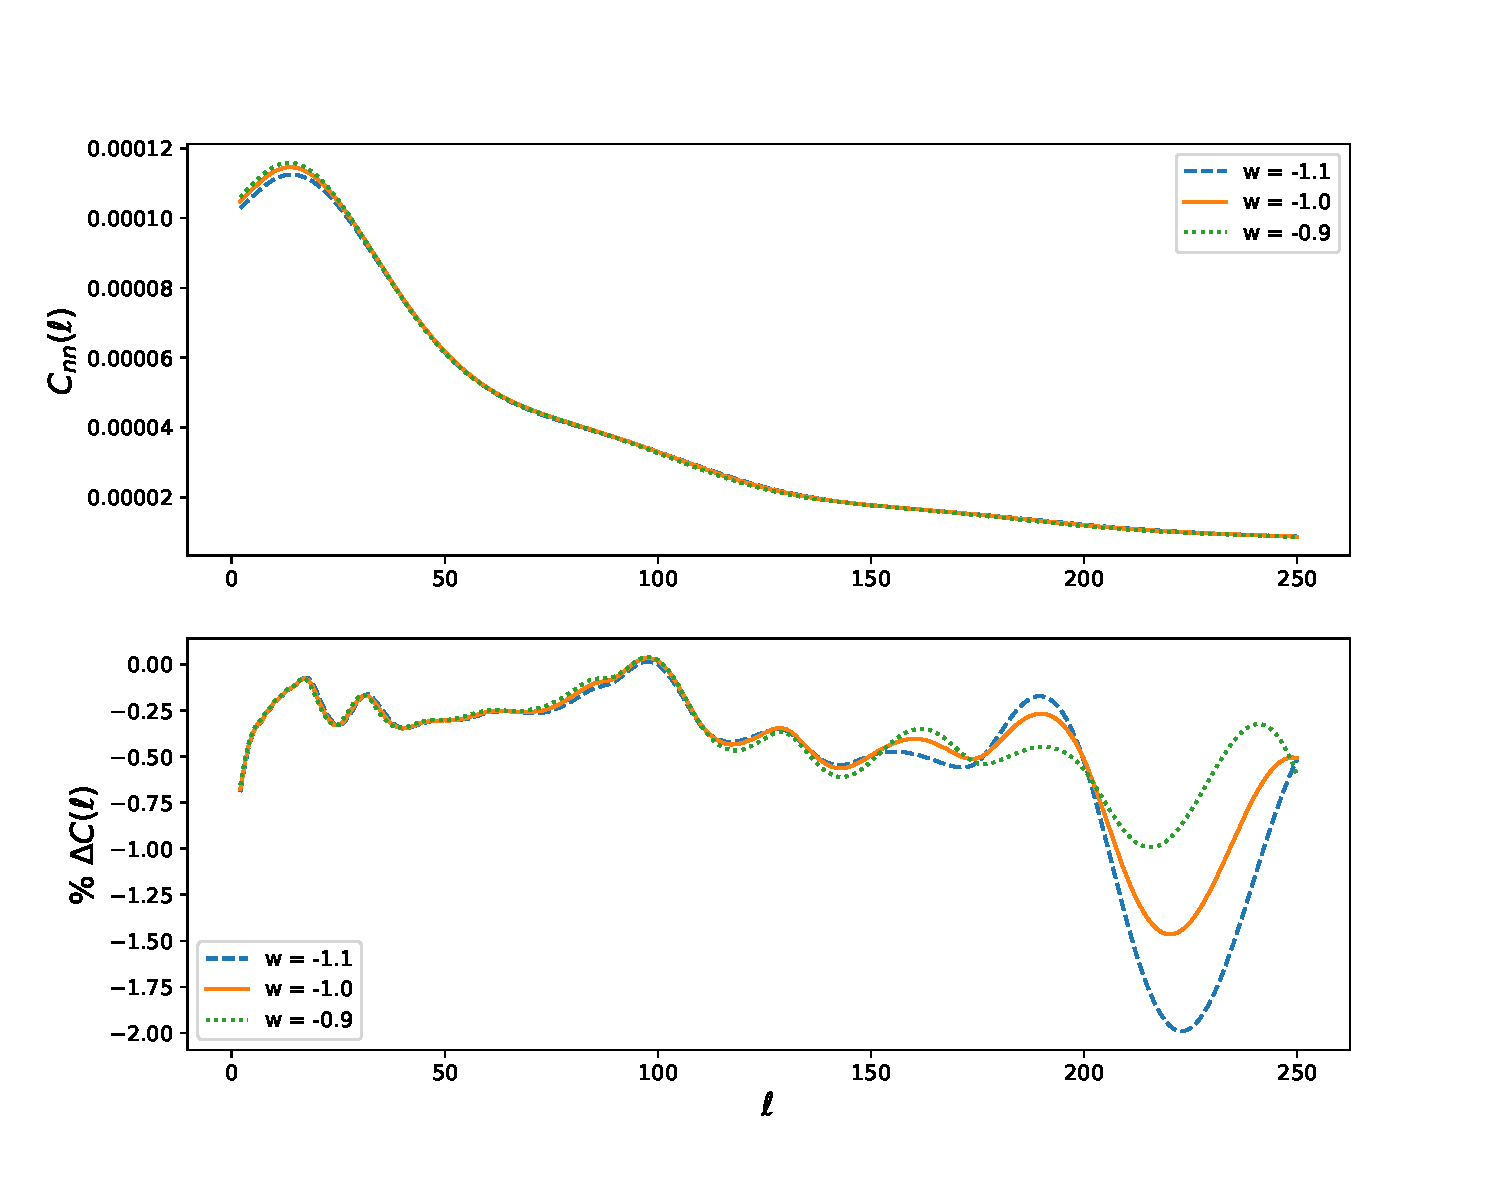
\includegraphics[scale=0.60]{BOSS-FIGS/PrecW.pdf}
\caption[Auto-correlations ($\bar z = 0.5$) for three values of $w$ calculated in \uclcl and comparison between \class and \texttt{CAMBSources}]{The top panel shows the auto-correlations ($\bar z = 0.5$) for three values of $w$ calculated in \uclcl. The lower panel shows the percentage difference of each of these $C_{\ell}$s with the corresponding $C_{\ell}$s from \texttt{CAMBSources} (matching values of $w$).}
\label{fig:w_Precision}
\end{center}
\end{figure}

\begin{figure}
\begin{center}
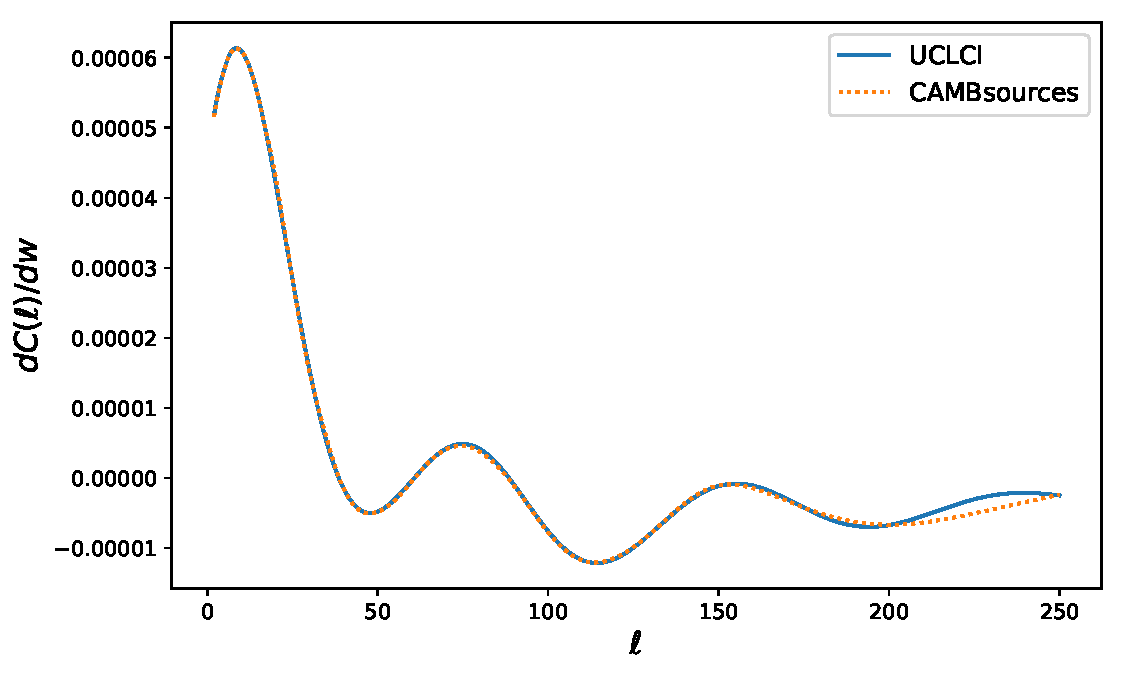
\includegraphics[scale=0.60]{BOSS-FIGS/PrecDw.pdf}
\caption[Comparison of $C_{\ell}$ derivatives $\frac{d C_{\ell}}{dw}$ between \uclcl and \texttt{CAMBSources}.]{Comparison of $C_{\ell}$ derivatives $\frac{d C_{\ell}}{dw}$ between \uclcl and \texttt{CAMBSources}. Here we see a more significant difference at high $\ell$, which can also been seen in Figure \ref{fig:w_Precision}. This characteristic bump appears to come from a difference in the \class and \texttt{CAMBSources} non-linear perturbations.}
\label{fig:Diff_w}
\end{center}
\end{figure}



\section{Full Systematics Analysis}\label{Apx:Systematics}
I show in this appendix the full cross correlation analysis I have performed in order to confirm that there is no strong evidence for systematic effects which would bias the power spectrum analysis. I do that by cross-correlating selected redshift bins with the systematic maps we have produced. In Figure \ref{fig:SYS_Appendix1Map} we show all the systematic overdenstity maps, using the CMASS mask as an example, created as mentioned in Section \ref{Sec:SystMaps}. I have already shown these results for one of the bins in the body of the text of Chapter \ref{Chap:BOSS} and, for clarity, I show here, in Figures \ref{fig:SystBin0}, \ref{fig:SystBin1}, \ref{fig:SystBin2}, \ref{fig:SystBin4}, \ref{fig:SystBin5}, and \ref{fig:SystBin6} the remaining cross-power spectra.

\begin{figure*}
\begin{subfigure}{.33\textwidth}
  \centering
    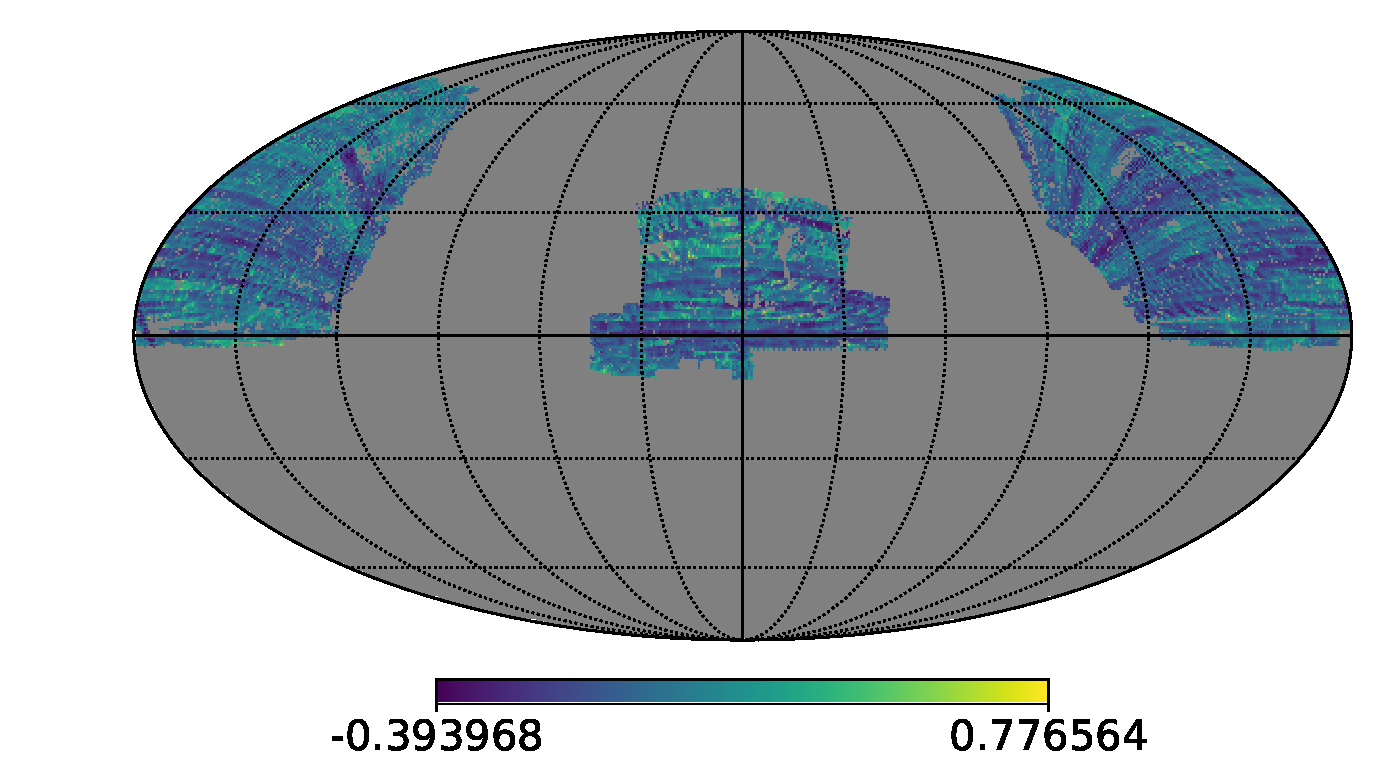
\includegraphics[scale=0.214]{SystematicMaps2/map_sdss_dr12_systematics_psffwhmu.pdf}
	\label{fig:systmap0}
    \caption{PSF FWHM in \textit{u} band}
\end{subfigure}
\begin{subfigure}{.33\textwidth}
  \centering
	\centering
    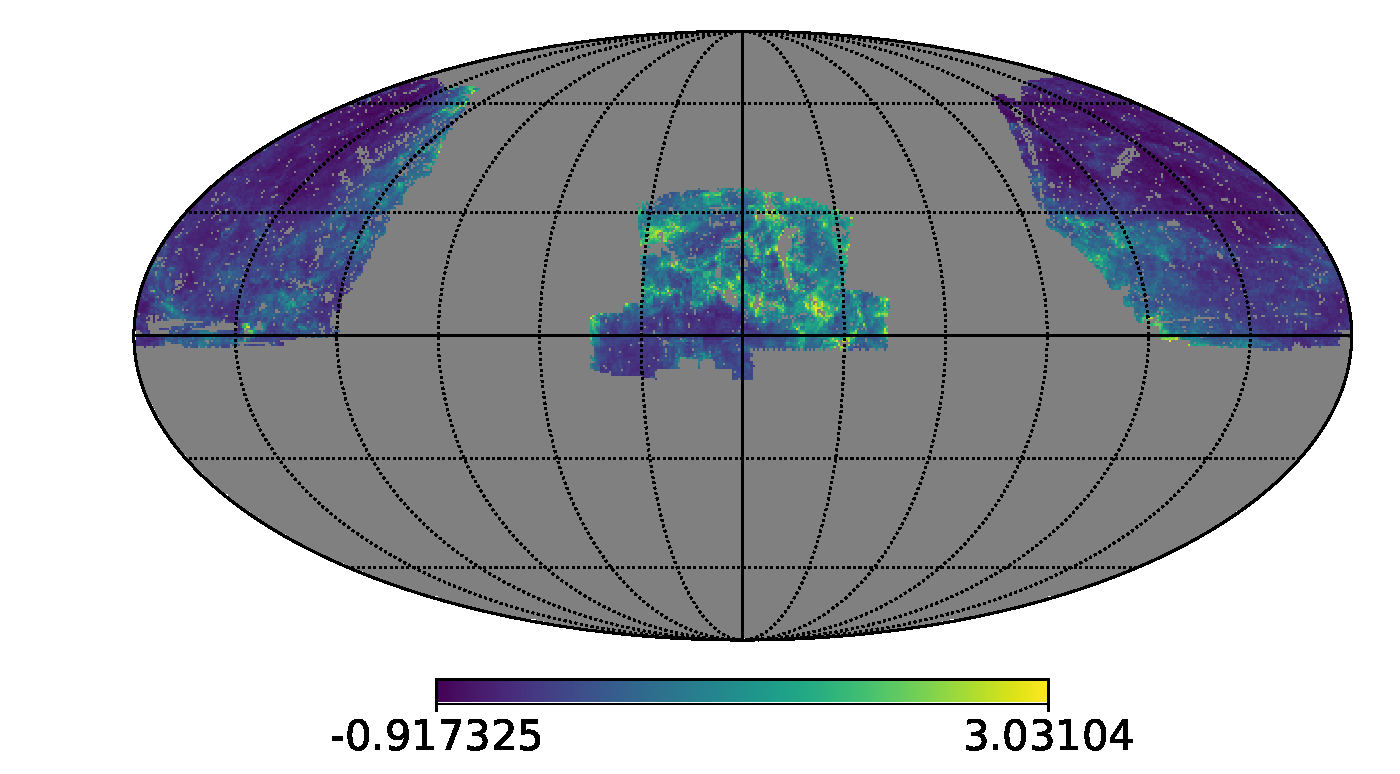
\includegraphics[scale=0.214]{SystematicMaps2/map_extinction_sfd-scaling_Overdensity_N512_cmassAll.pdf}
	\label{fig:systmap1}
    \caption{SFD scaling}
\end{subfigure}
\begin{subfigure}{.33\textwidth}
  \centering
	\centering
    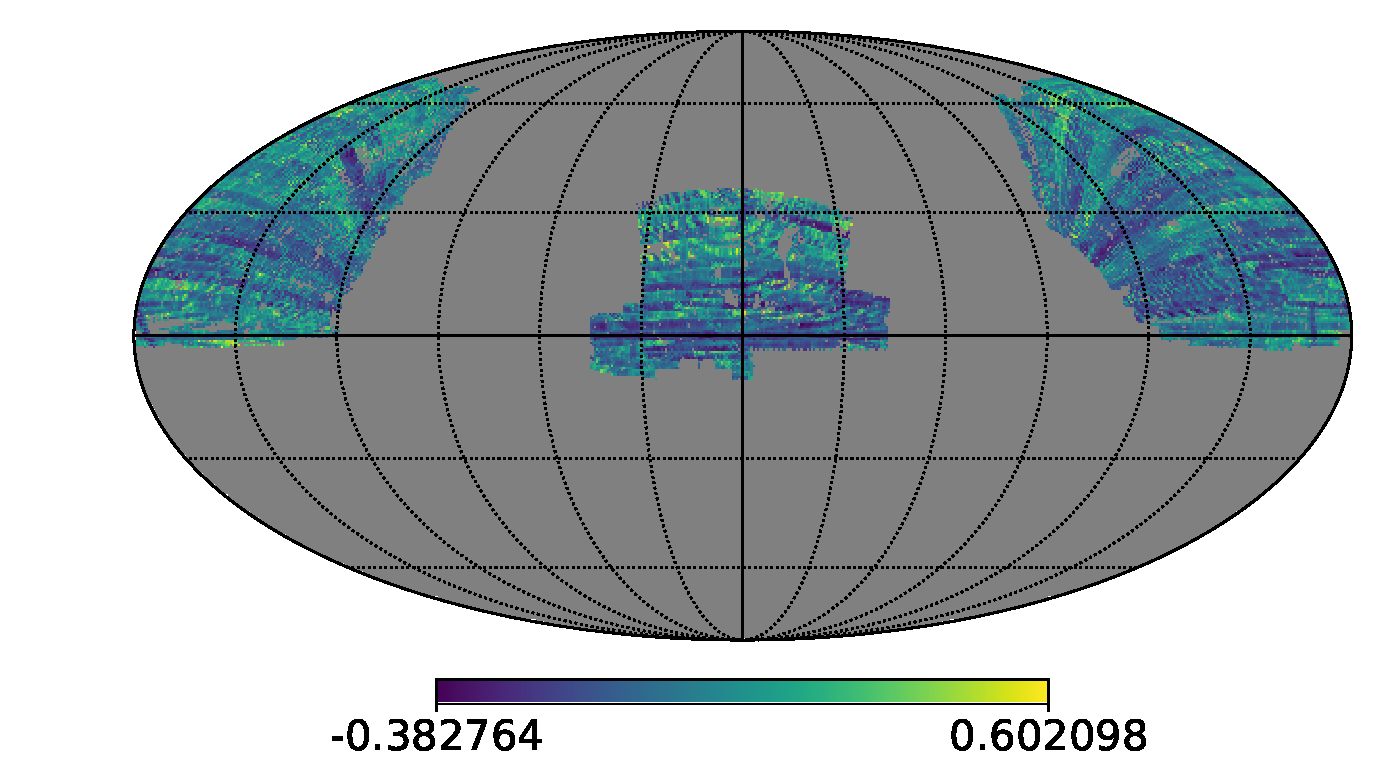
\includegraphics[scale=0.214]{SystematicMaps2/map_sdss_dr12_systematics_psffwhmr.pdf}
	\label{fig:systmap2}
    \caption{PSF FWHM in \textit{r} band}
\end{subfigure}
\\
\begin{subfigure}{.33\textwidth}
  \centering
	\centering
    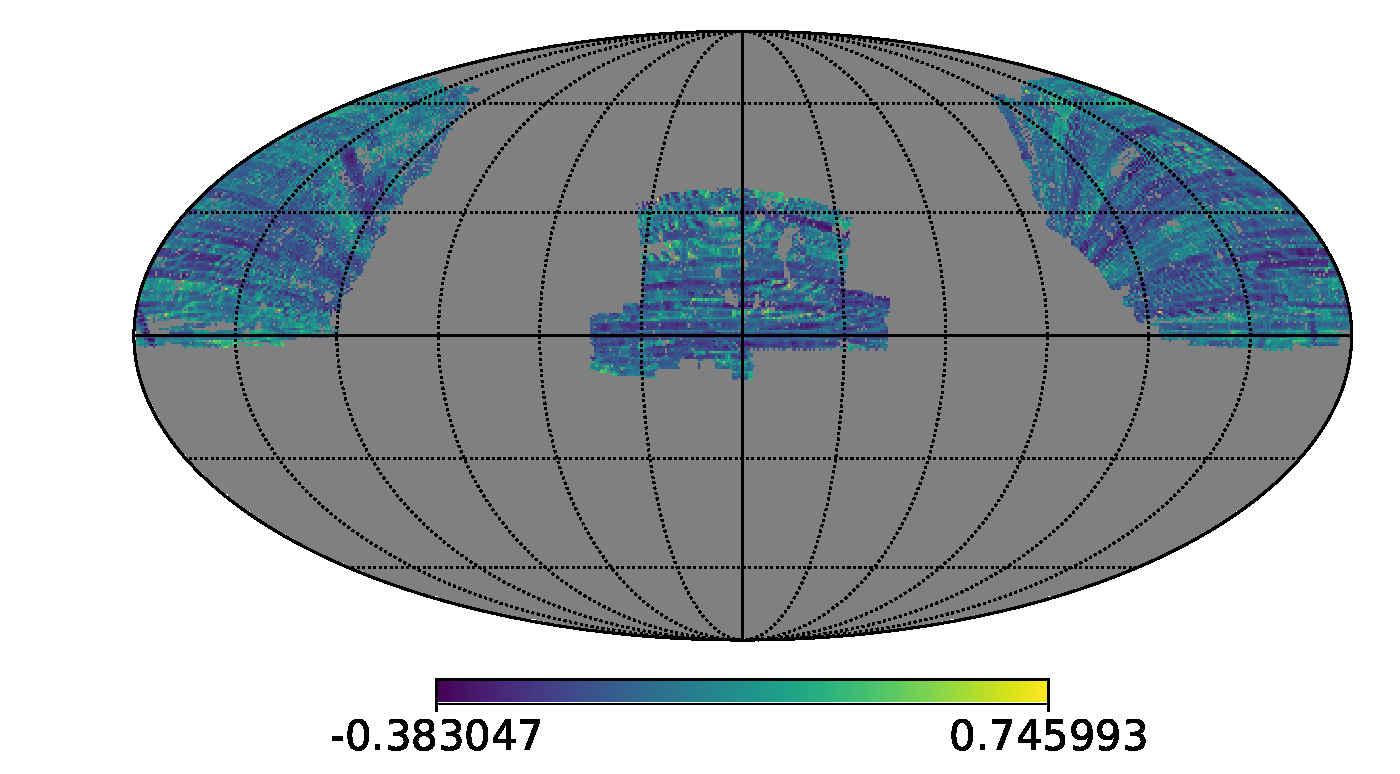
\includegraphics[scale=0.214]{SystematicMaps2/map_sdss_dr12_systematics_psffwhmz.pdf}
	\label{fig:systmap4}
    \caption{PSF FWHM in \textit{z} band}
\end{subfigure}
\begin{subfigure}{.33\textwidth}
  \centering
	\centering
    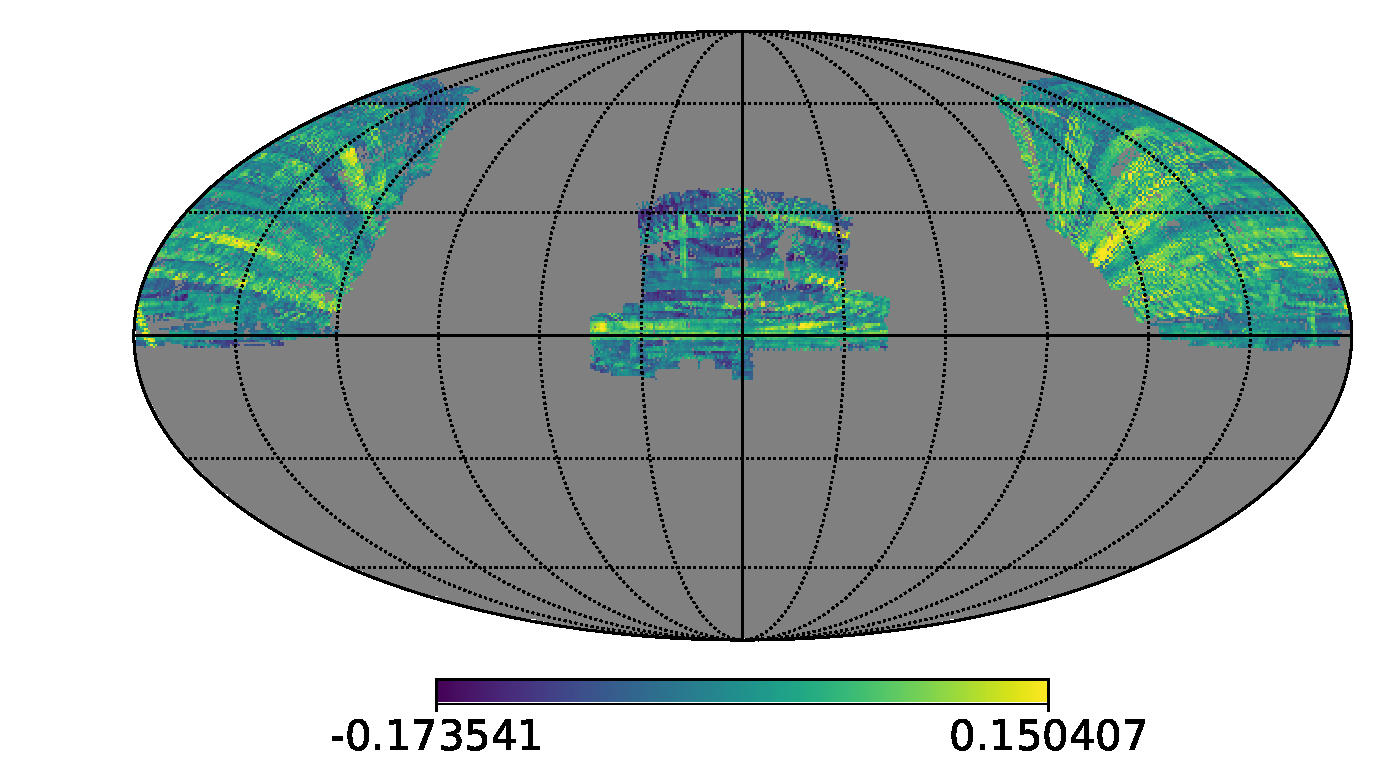
\includegraphics[scale=0.214]{SystematicMaps2/map_sdss_dr12_systematics_score.pdf}
    \label{fig:systmap5}
    \caption{SDSS score}
\end{subfigure}
\begin{subfigure}{.33\textwidth}
  \centering
	\centering
    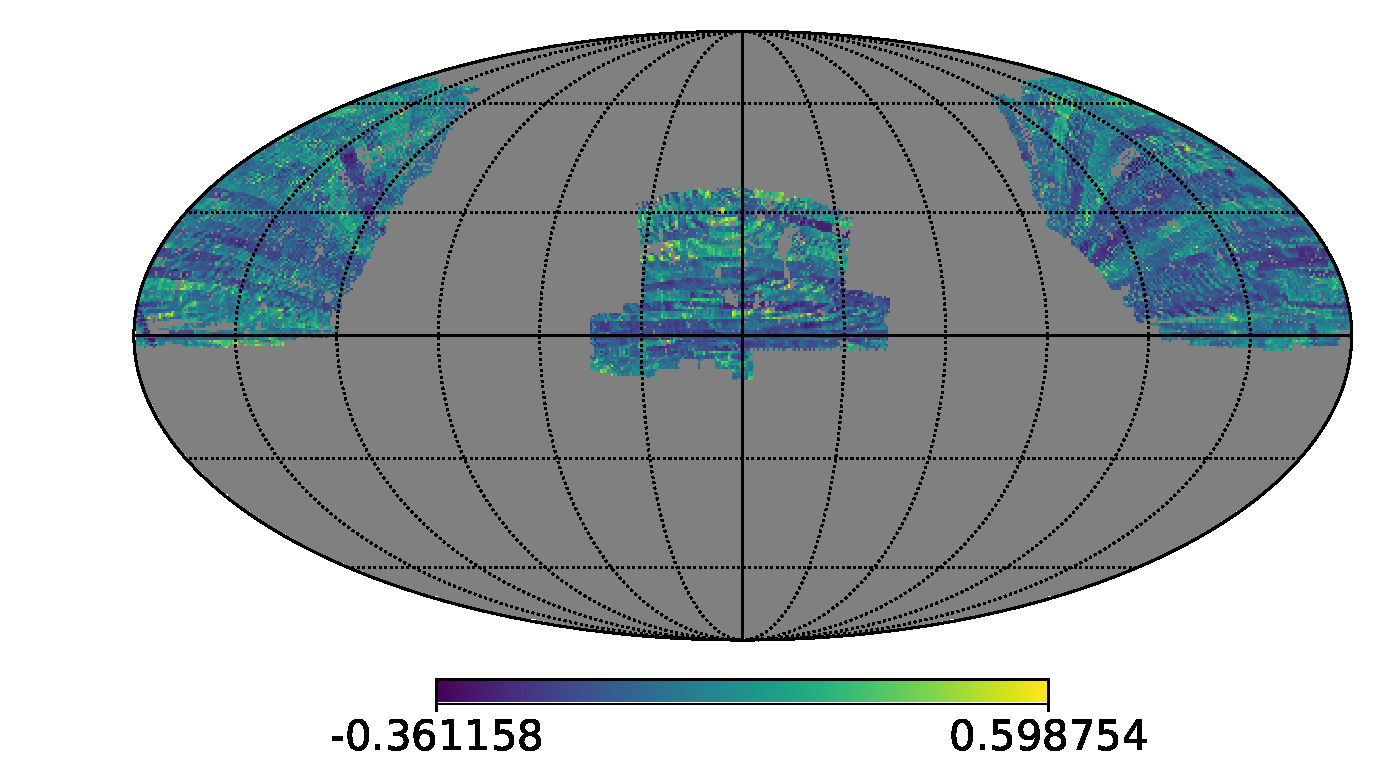
\includegraphics[scale=0.214]{SystematicMaps2/map_sdss_dr12_systematics_psffwhmg.pdf}
	\label{fig:systmap6}
    \caption{PSF FWHM in \textit{g} band}
\end{subfigure}
\\
\begin{subfigure}{.33\textwidth}
  \centering
    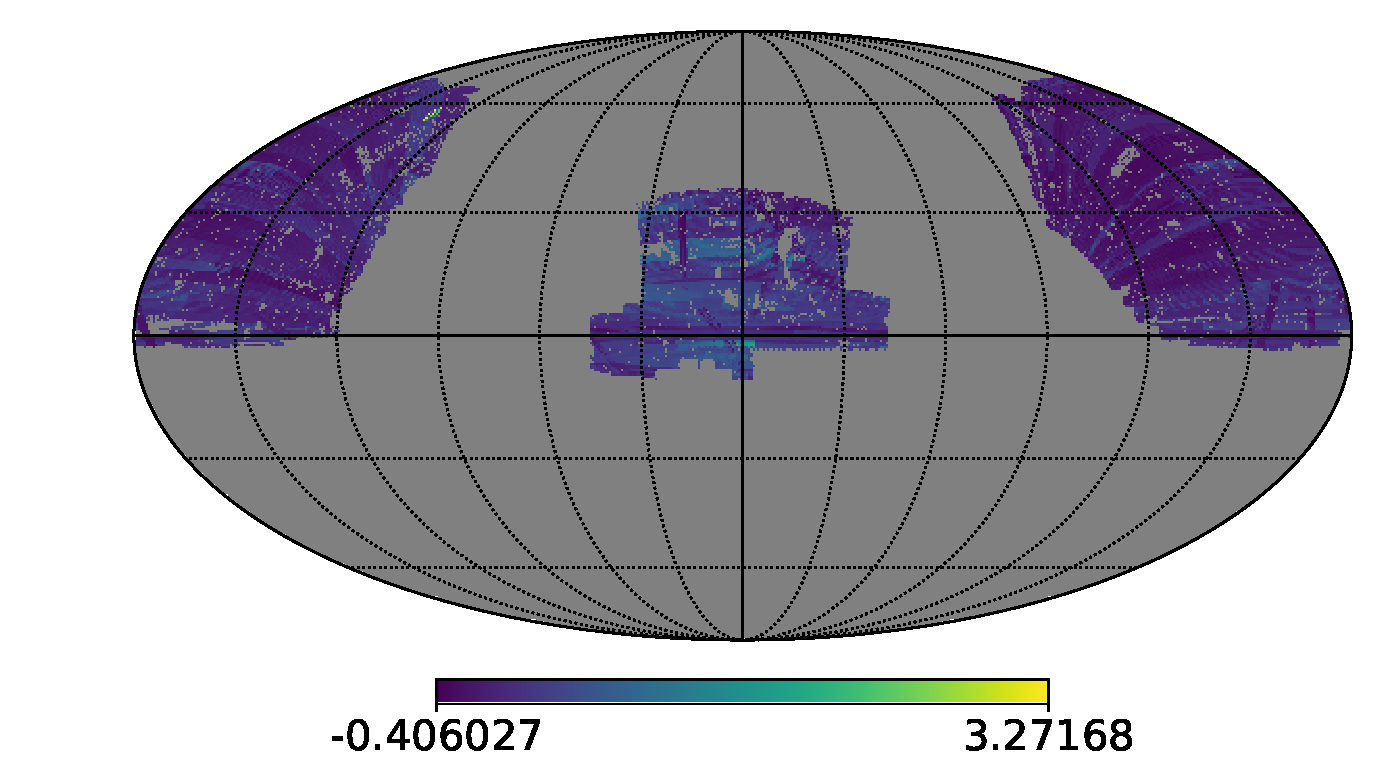
\includegraphics[scale=0.214]{SystematicMaps2/map_sdss_dr12_systematics_skyfluxg.pdf}
    \label{fig:systmap7}
    \caption{sky flux in \textit{g} band}
\end{subfigure}
\begin{subfigure}{.33\textwidth}
  \centering
    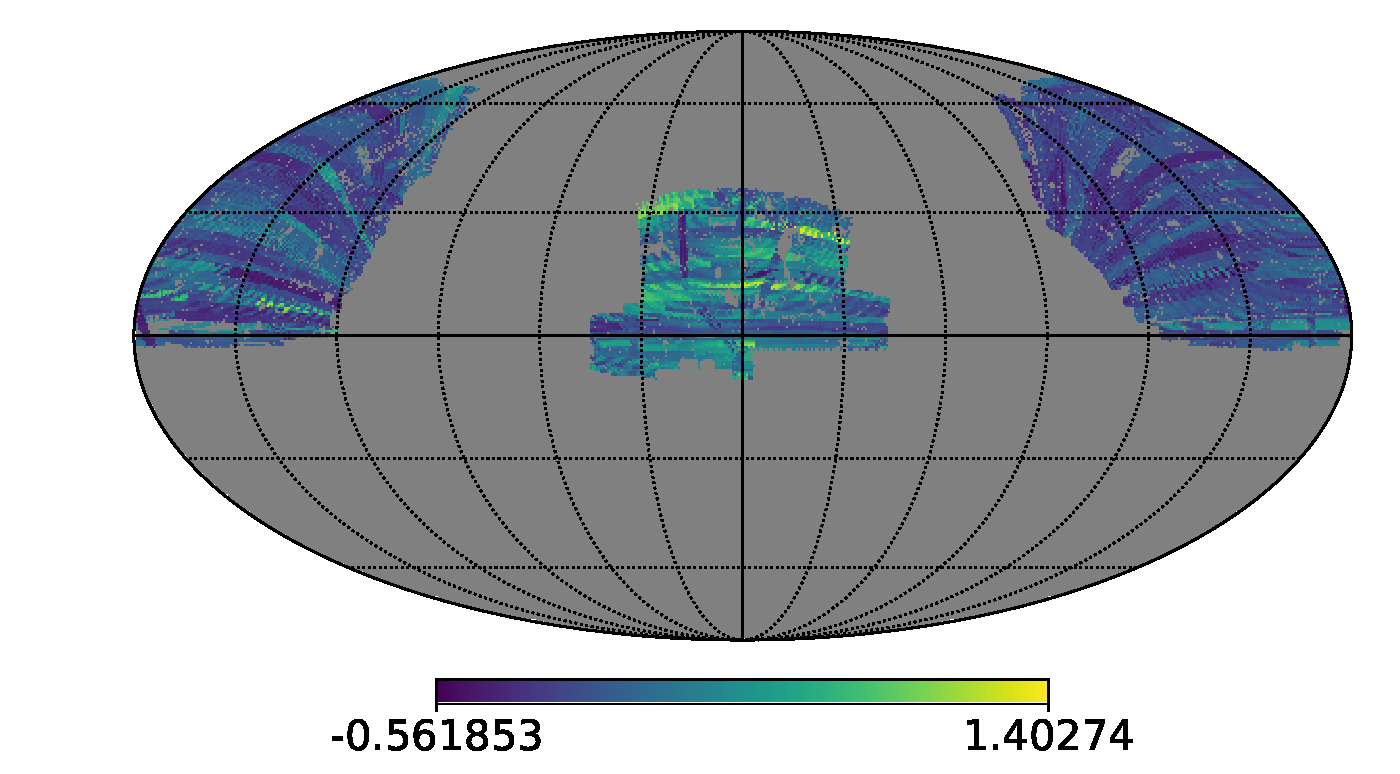
\includegraphics[scale=0.214]{SystematicMaps2/map_sdss_dr12_systematics_skyfluxi.pdf}
    \label{fig:systmap8}
    \caption{sky flux in \textit{i} band}
\end{subfigure}
\begin{subfigure}{.33\textwidth}
  \centering
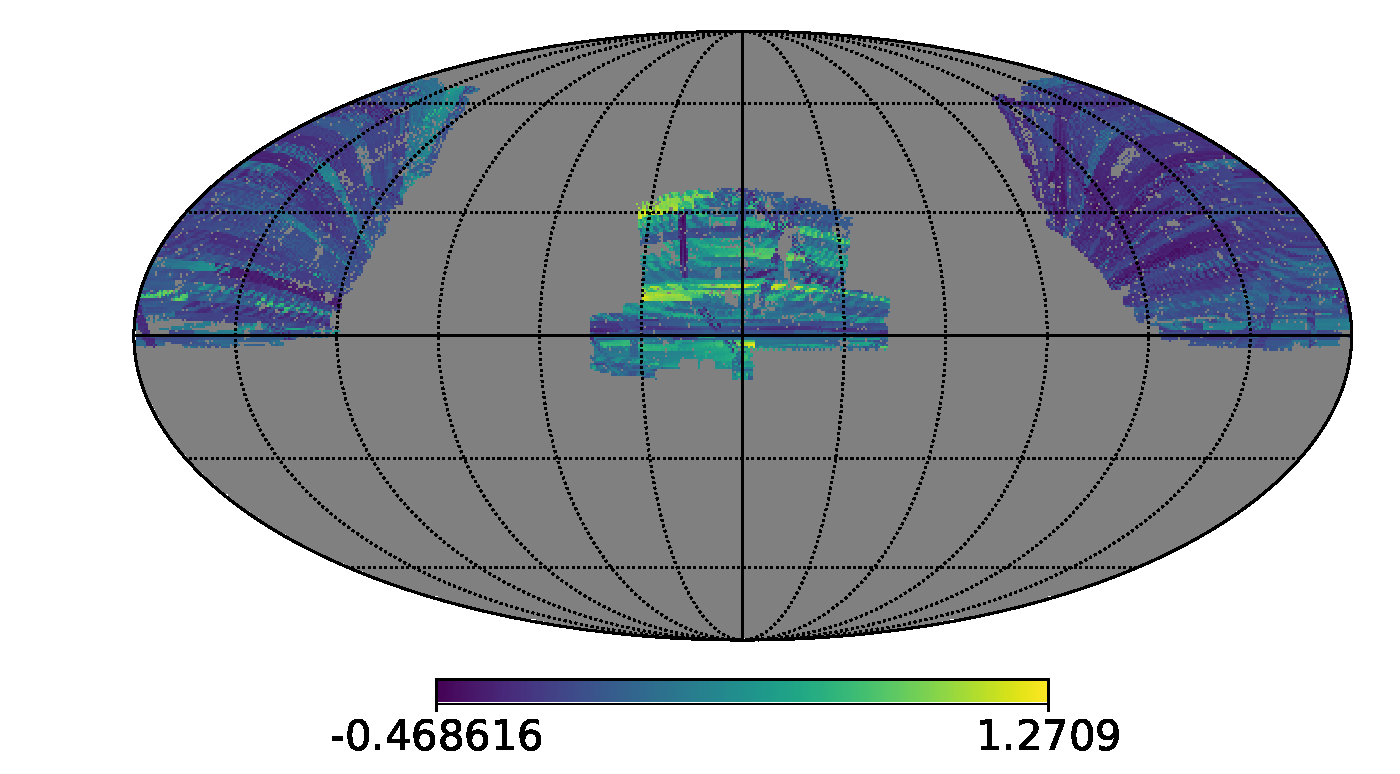
\includegraphics[scale=0.214]{SystematicMaps2/map_sdss_dr12_systematics_skyfluxr.pdf}
\label{fig:systmap9}
    \caption{sky flux in \textit{r} band}
\end{subfigure}
\\
\begin{subfigure}{.33\textwidth}
  \centering
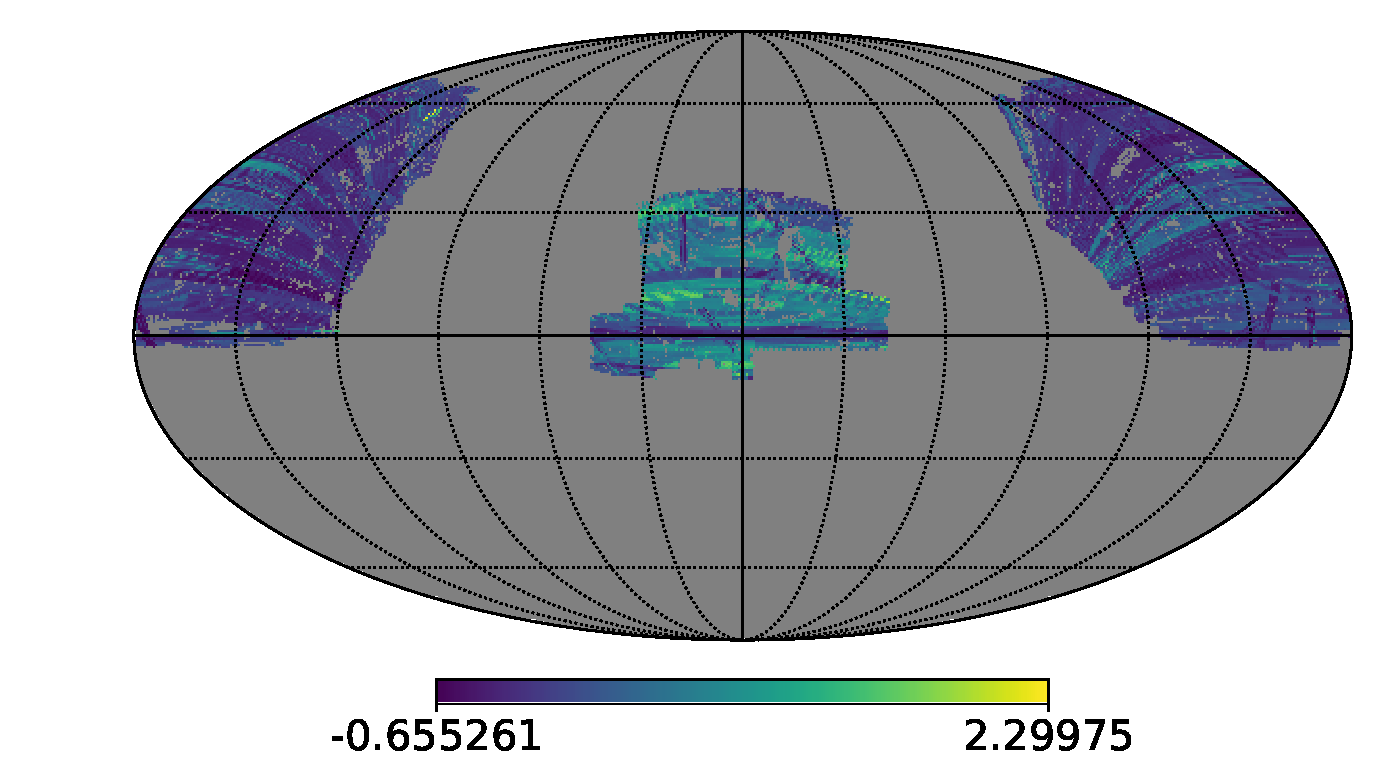
\includegraphics[scale=0.214]{SystematicMaps2/map_sdss_dr12_systematics_skyfluxu.pdf}
\label{fig:systmap10}
    \caption{sky flux in \textit{u} band}
\end{subfigure}
\begin{subfigure}{.33\textwidth}
  \centering
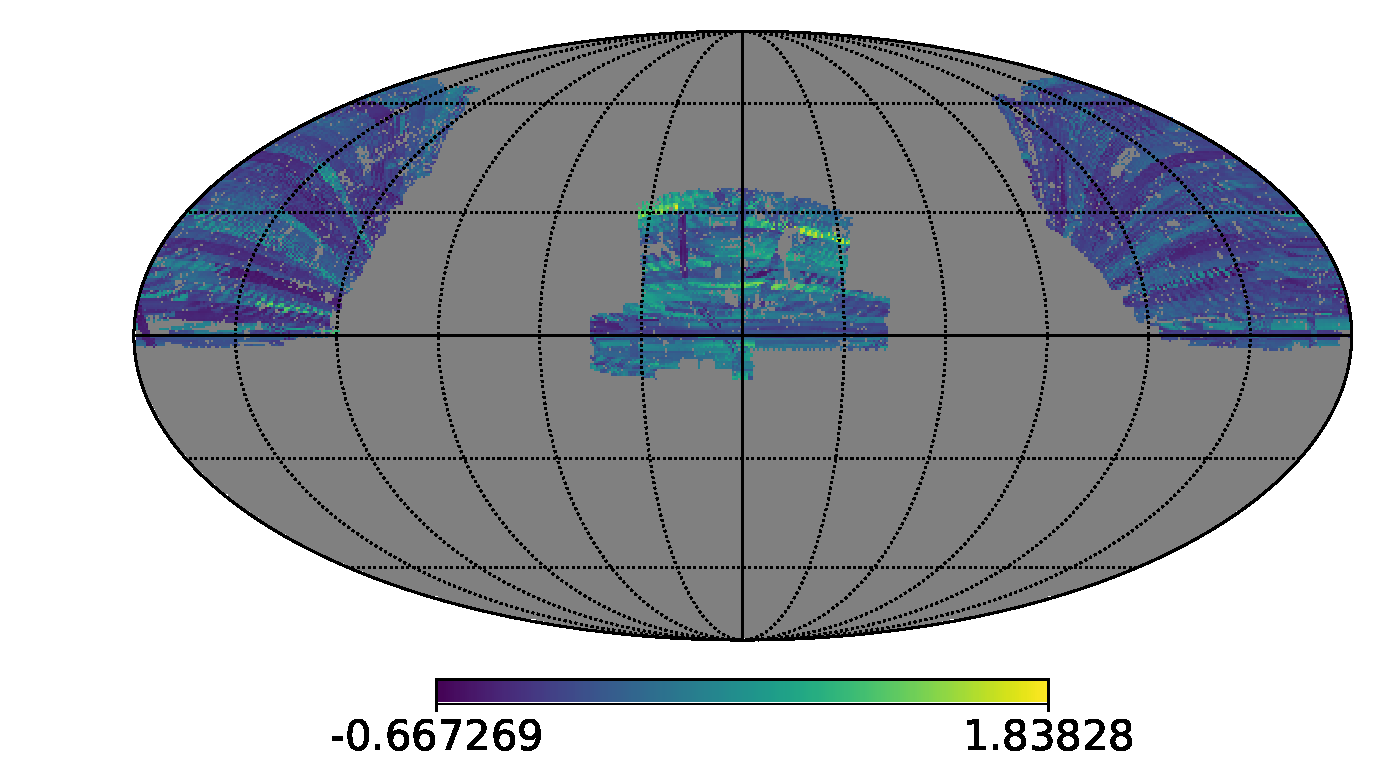
\includegraphics[scale=0.214]{SystematicMaps2/map_sdss_dr12_systematics_skyfluxz.pdf}
\label{fig:systmap11}
    \caption{sky flux in \textit{z} band}
\end{subfigure}
\begin{subfigure}{.33\textwidth}
  \centering
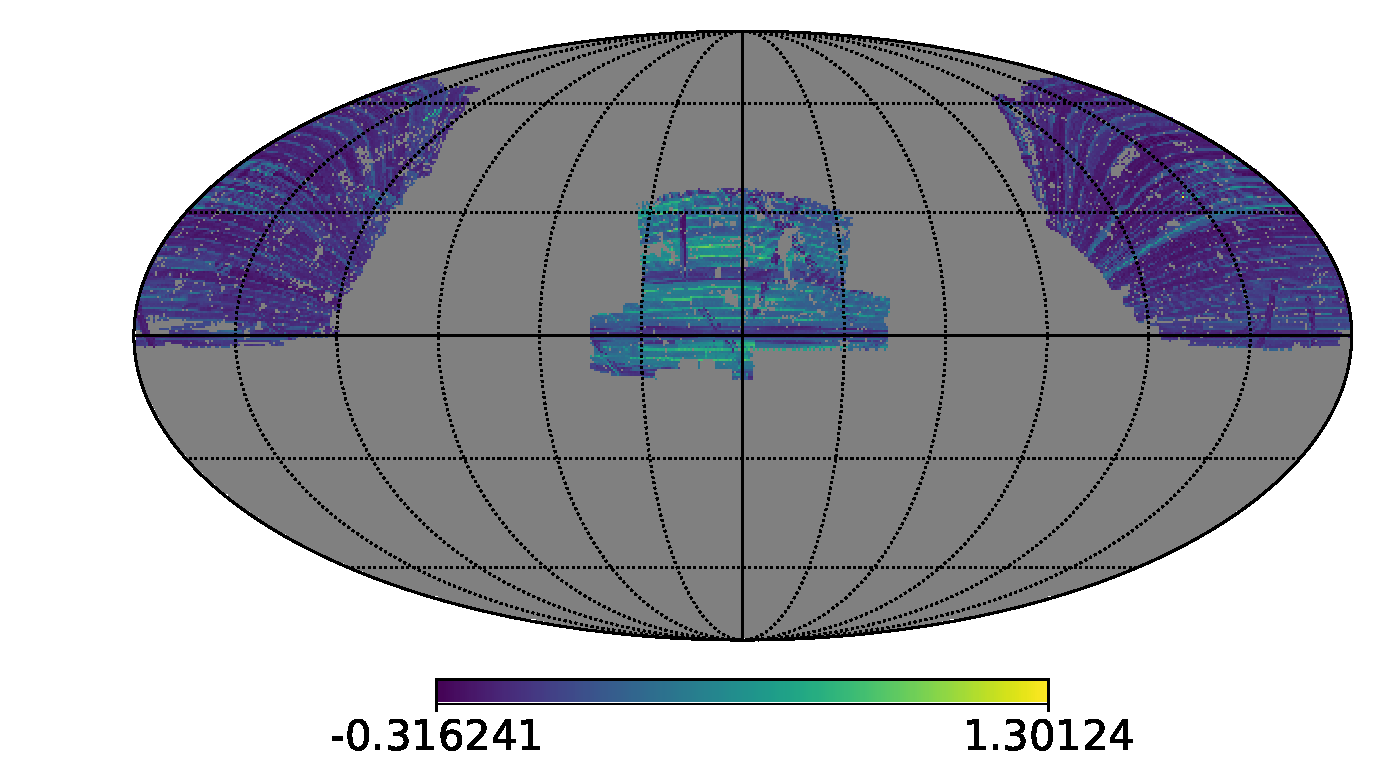
\includegraphics[scale=0.214]{SystematicMaps2/map_sdss_dr12_systematics_skysigmag.pdf}
\label{fig:systmap12}
    \caption{sky flux variance in \textit{g} band}
\end{subfigure}
\\
\begin{subfigure}{.33\textwidth}
  \centering
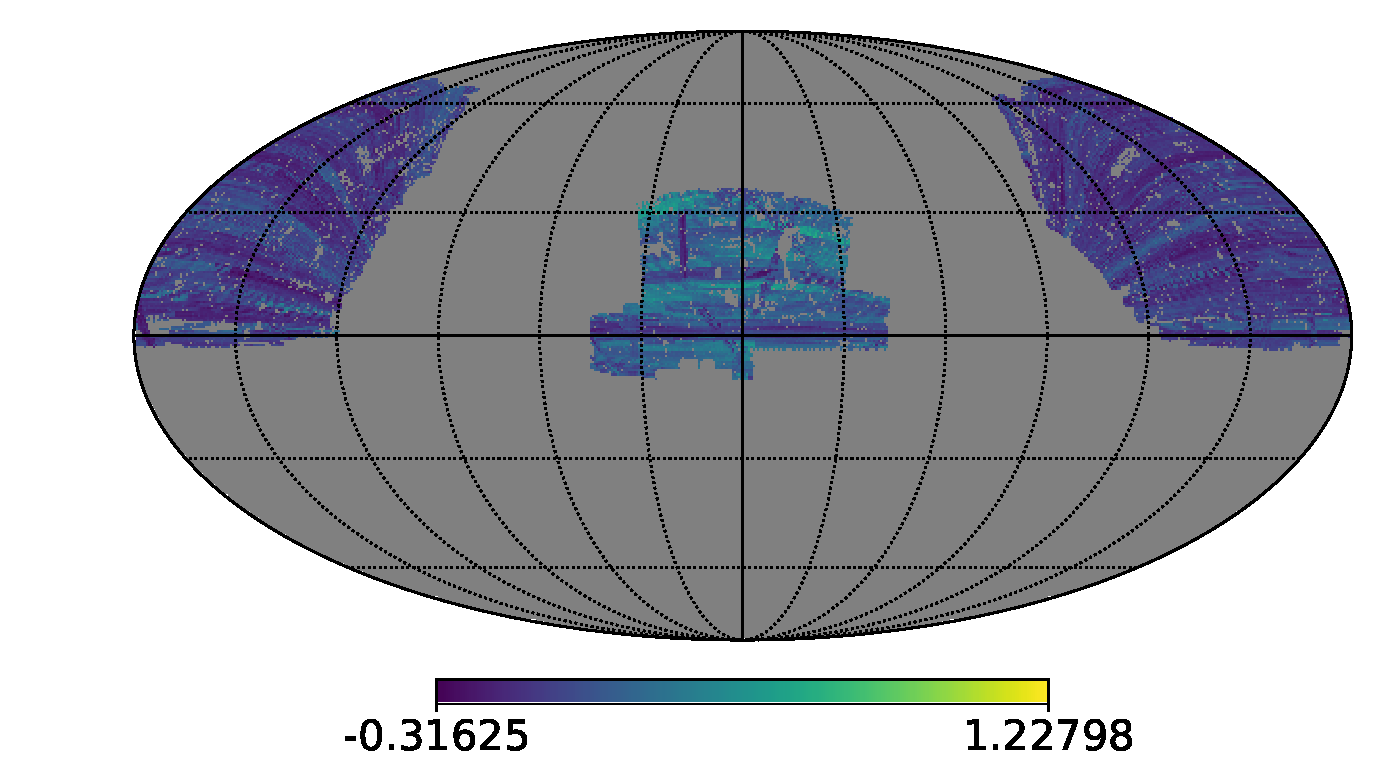
\includegraphics[scale=0.214]{SystematicMaps2/map_sdss_dr12_systematics_skysigmai.pdf}
\label{fig:systmap13}
    \caption{sky flux variance in \textit{i} band}
\end{subfigure}
\begin{subfigure}{.33\textwidth}
  \centering
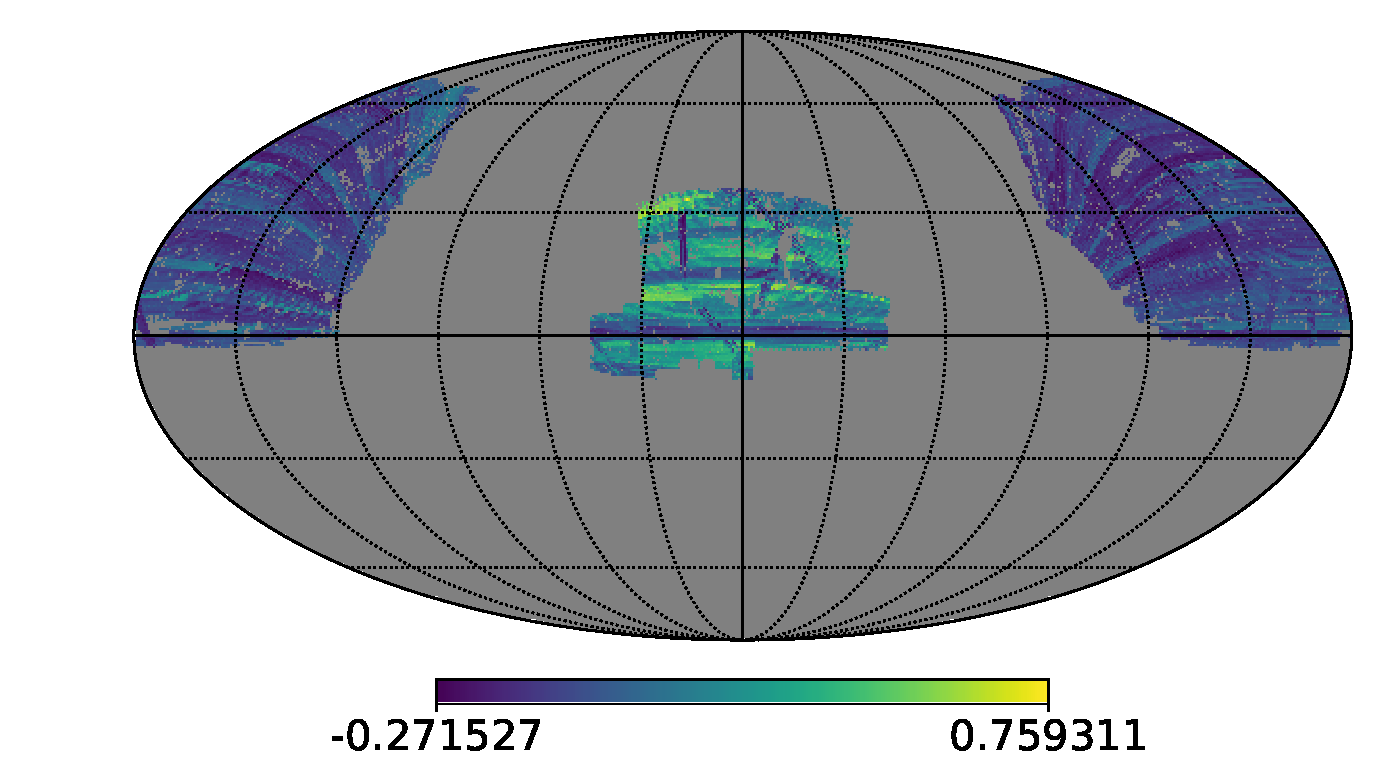
\includegraphics[scale=0.214]{SystematicMaps2/map_sdss_dr12_systematics_skysigmar.pdf}
\label{fig:systmap14}
    \caption{sky flux variance in \textit{r} band}
\end{subfigure}
\begin{subfigure}{.33\textwidth}
  \centering
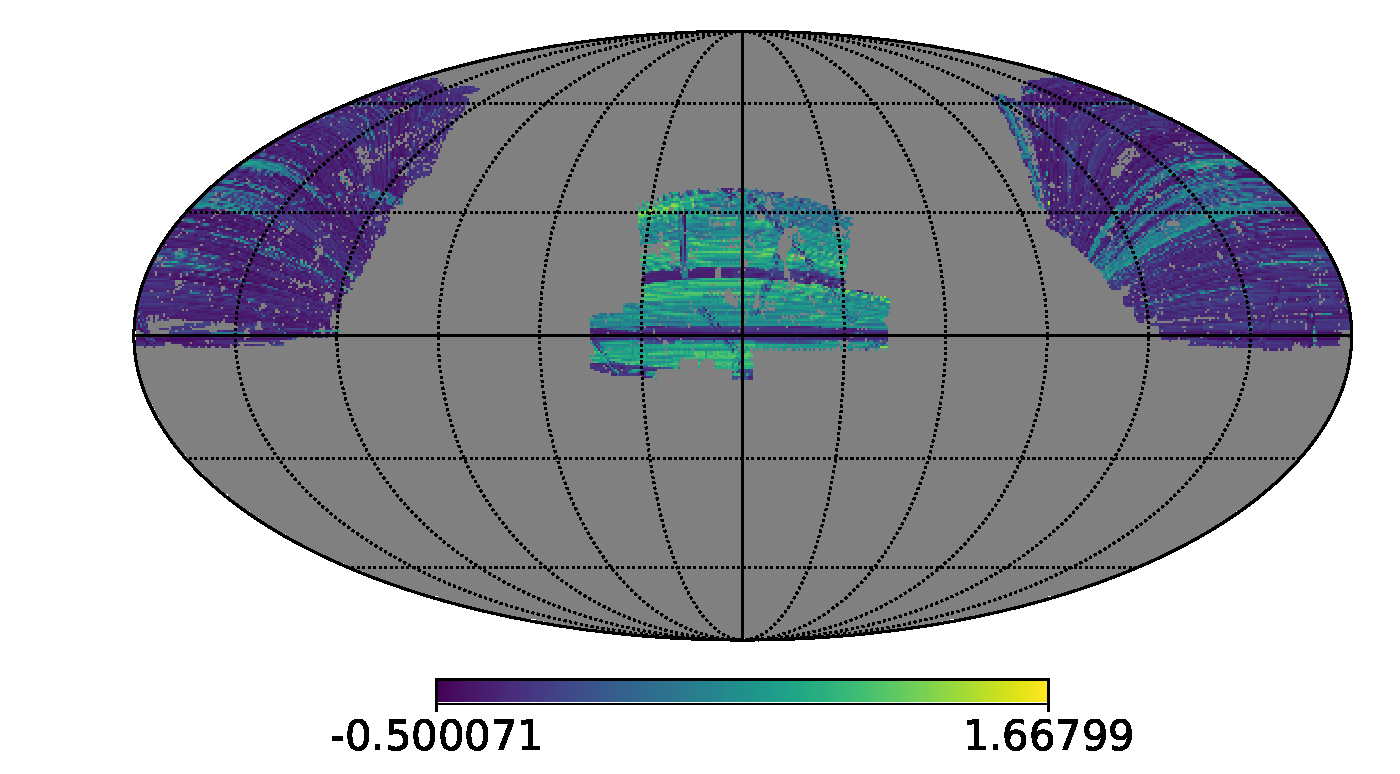
\includegraphics[scale=0.214]{SystematicMaps2/map_sdss_dr12_systematics_skysigmau.pdf}
\label{fig:systmap15}
    \caption{sky flux variance in \textit{u} band}
\end{subfigure}
\\
\begin{subfigure}{.33\textwidth}
  \centering
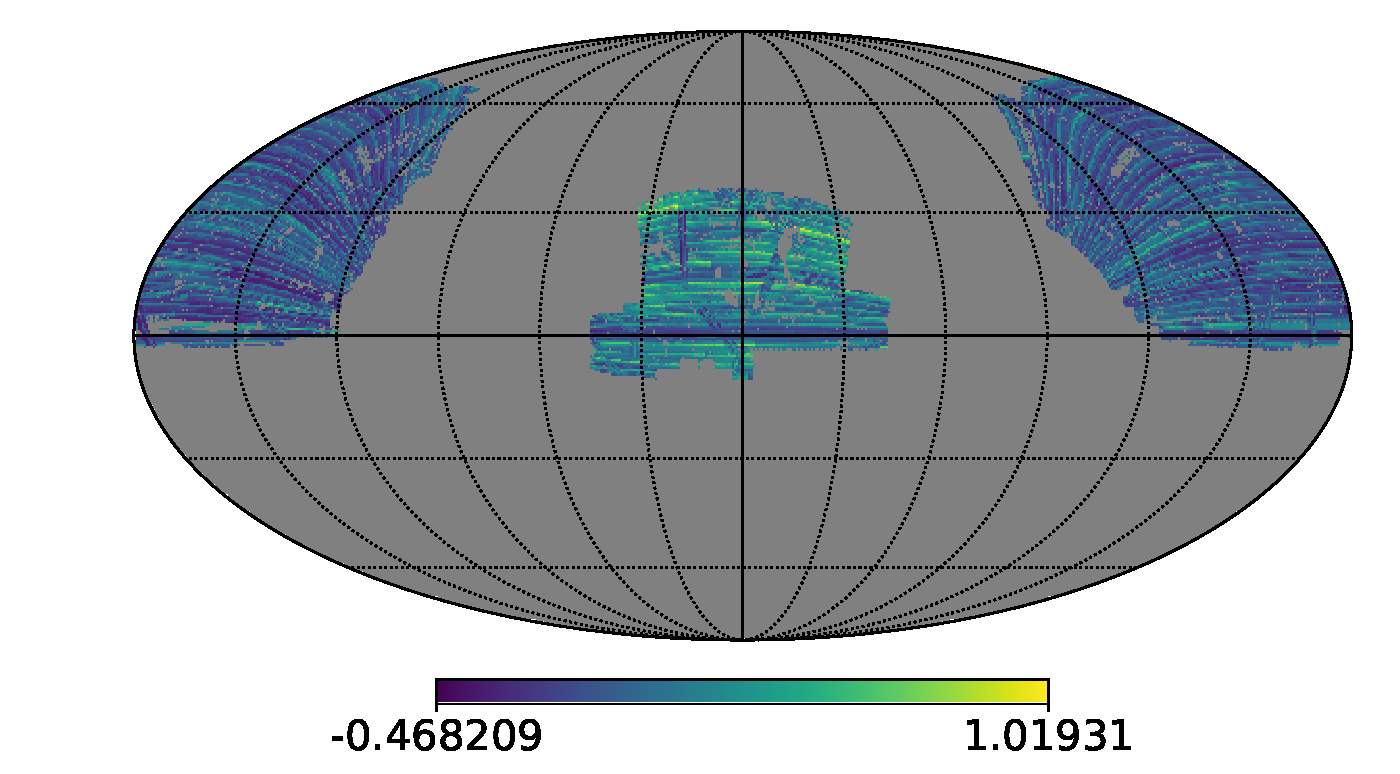
\includegraphics[scale=0.214]{SystematicMaps2/map_sdss_dr12_systematics_skysigmaz.pdf}
\label{fig:systmap16}
    \caption{sky flux variance in \textit{z} band}
\end{subfigure}
\begin{subfigure}{.33\textwidth}
  \centering
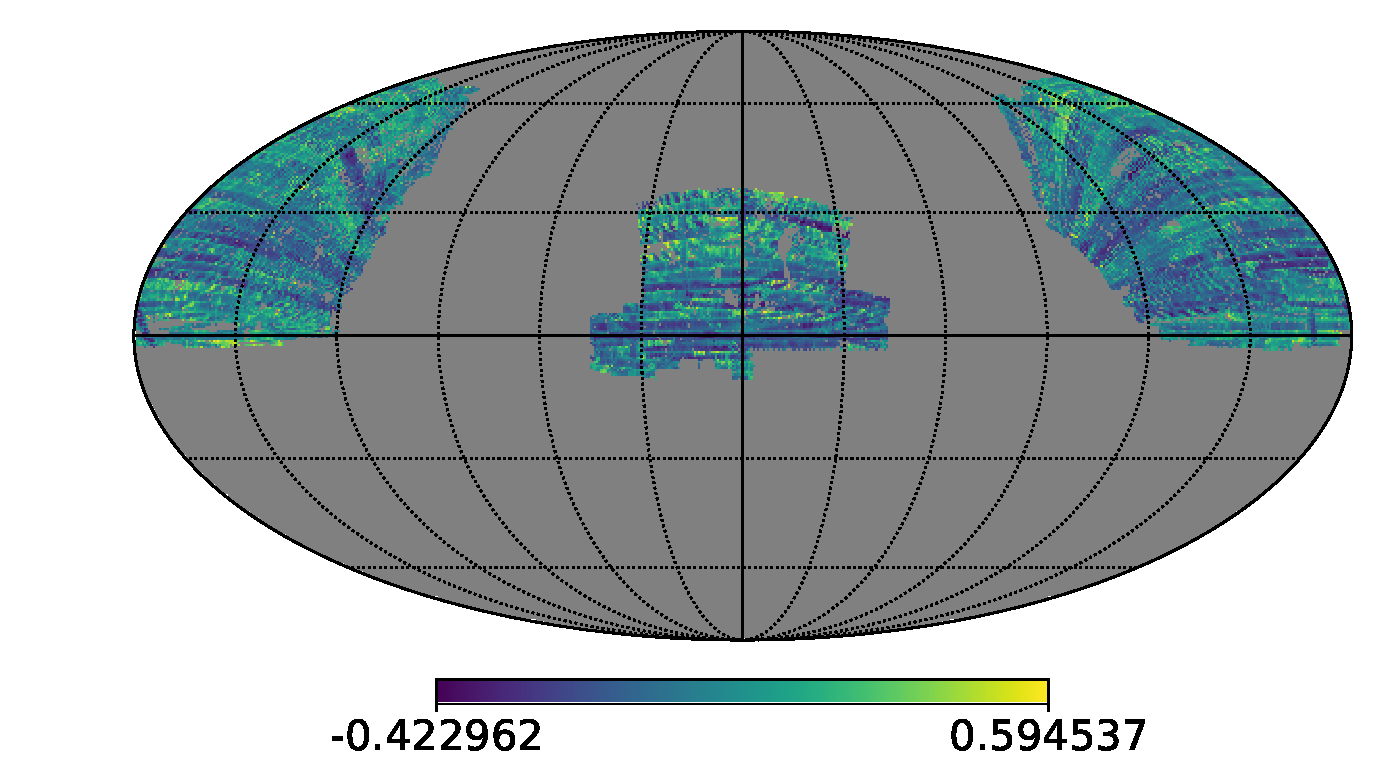
\includegraphics[scale=0.214]{SystematicMaps2/map_sdss_dr12_systematics_psffwhmi.pdf}
\label{fig:systmap17}
    \caption{PSF FWHM in \textit{i} band}
\end{subfigure}
\begin{subfigure}{.33\textwidth}
  \centering
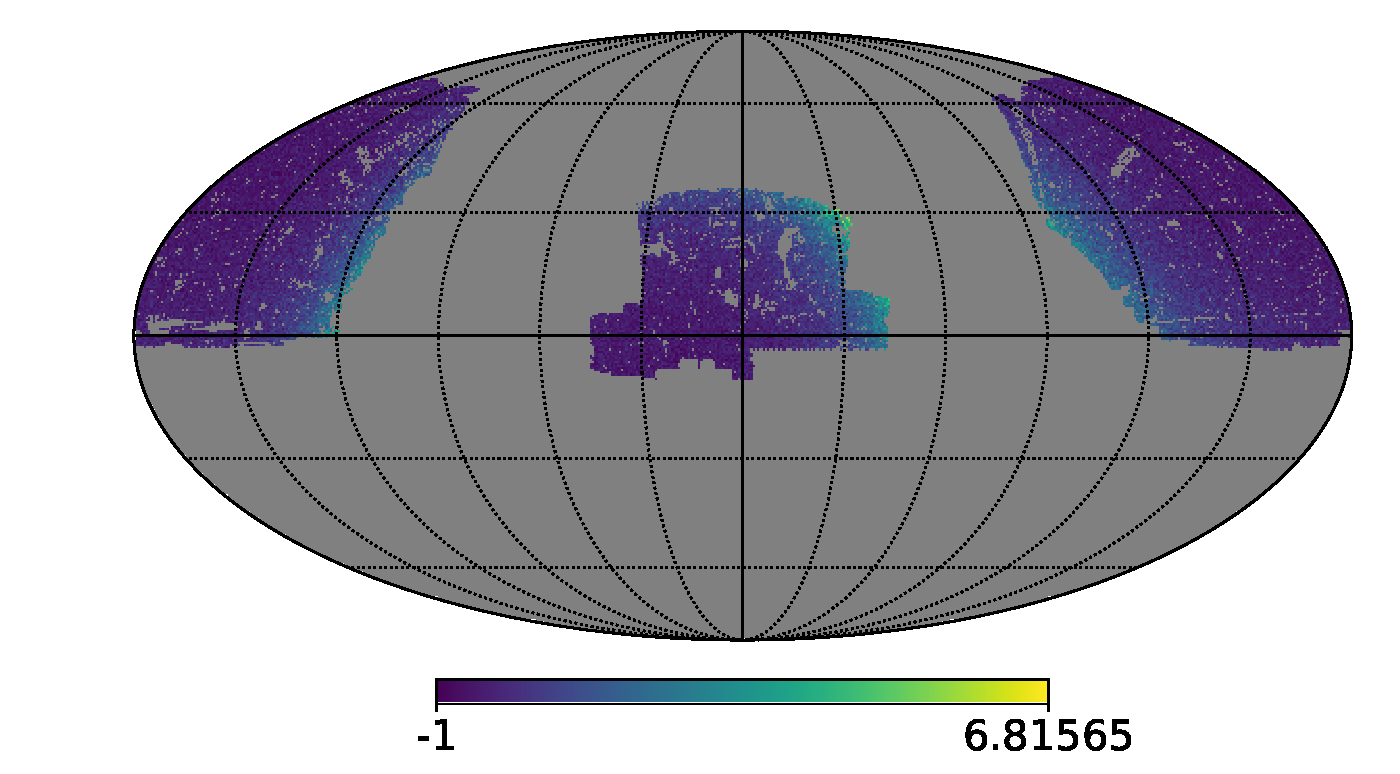
\includegraphics[scale=0.214]{SystematicMaps2/map_cmass_All_stellar_overdensity_N512.pdf}
\label{fig:systmap18}
    \caption{stellar overdensity}
\end{subfigure}
\caption[Systematic overdensity maps]{Systematic overdensity maps for the CMASS sample using the process described in Section \ref{Sec:SystMaps}.}
\label{fig:SYS_Appendix1Map}
\end{figure*}

\begin{figure*}
\begin{center}
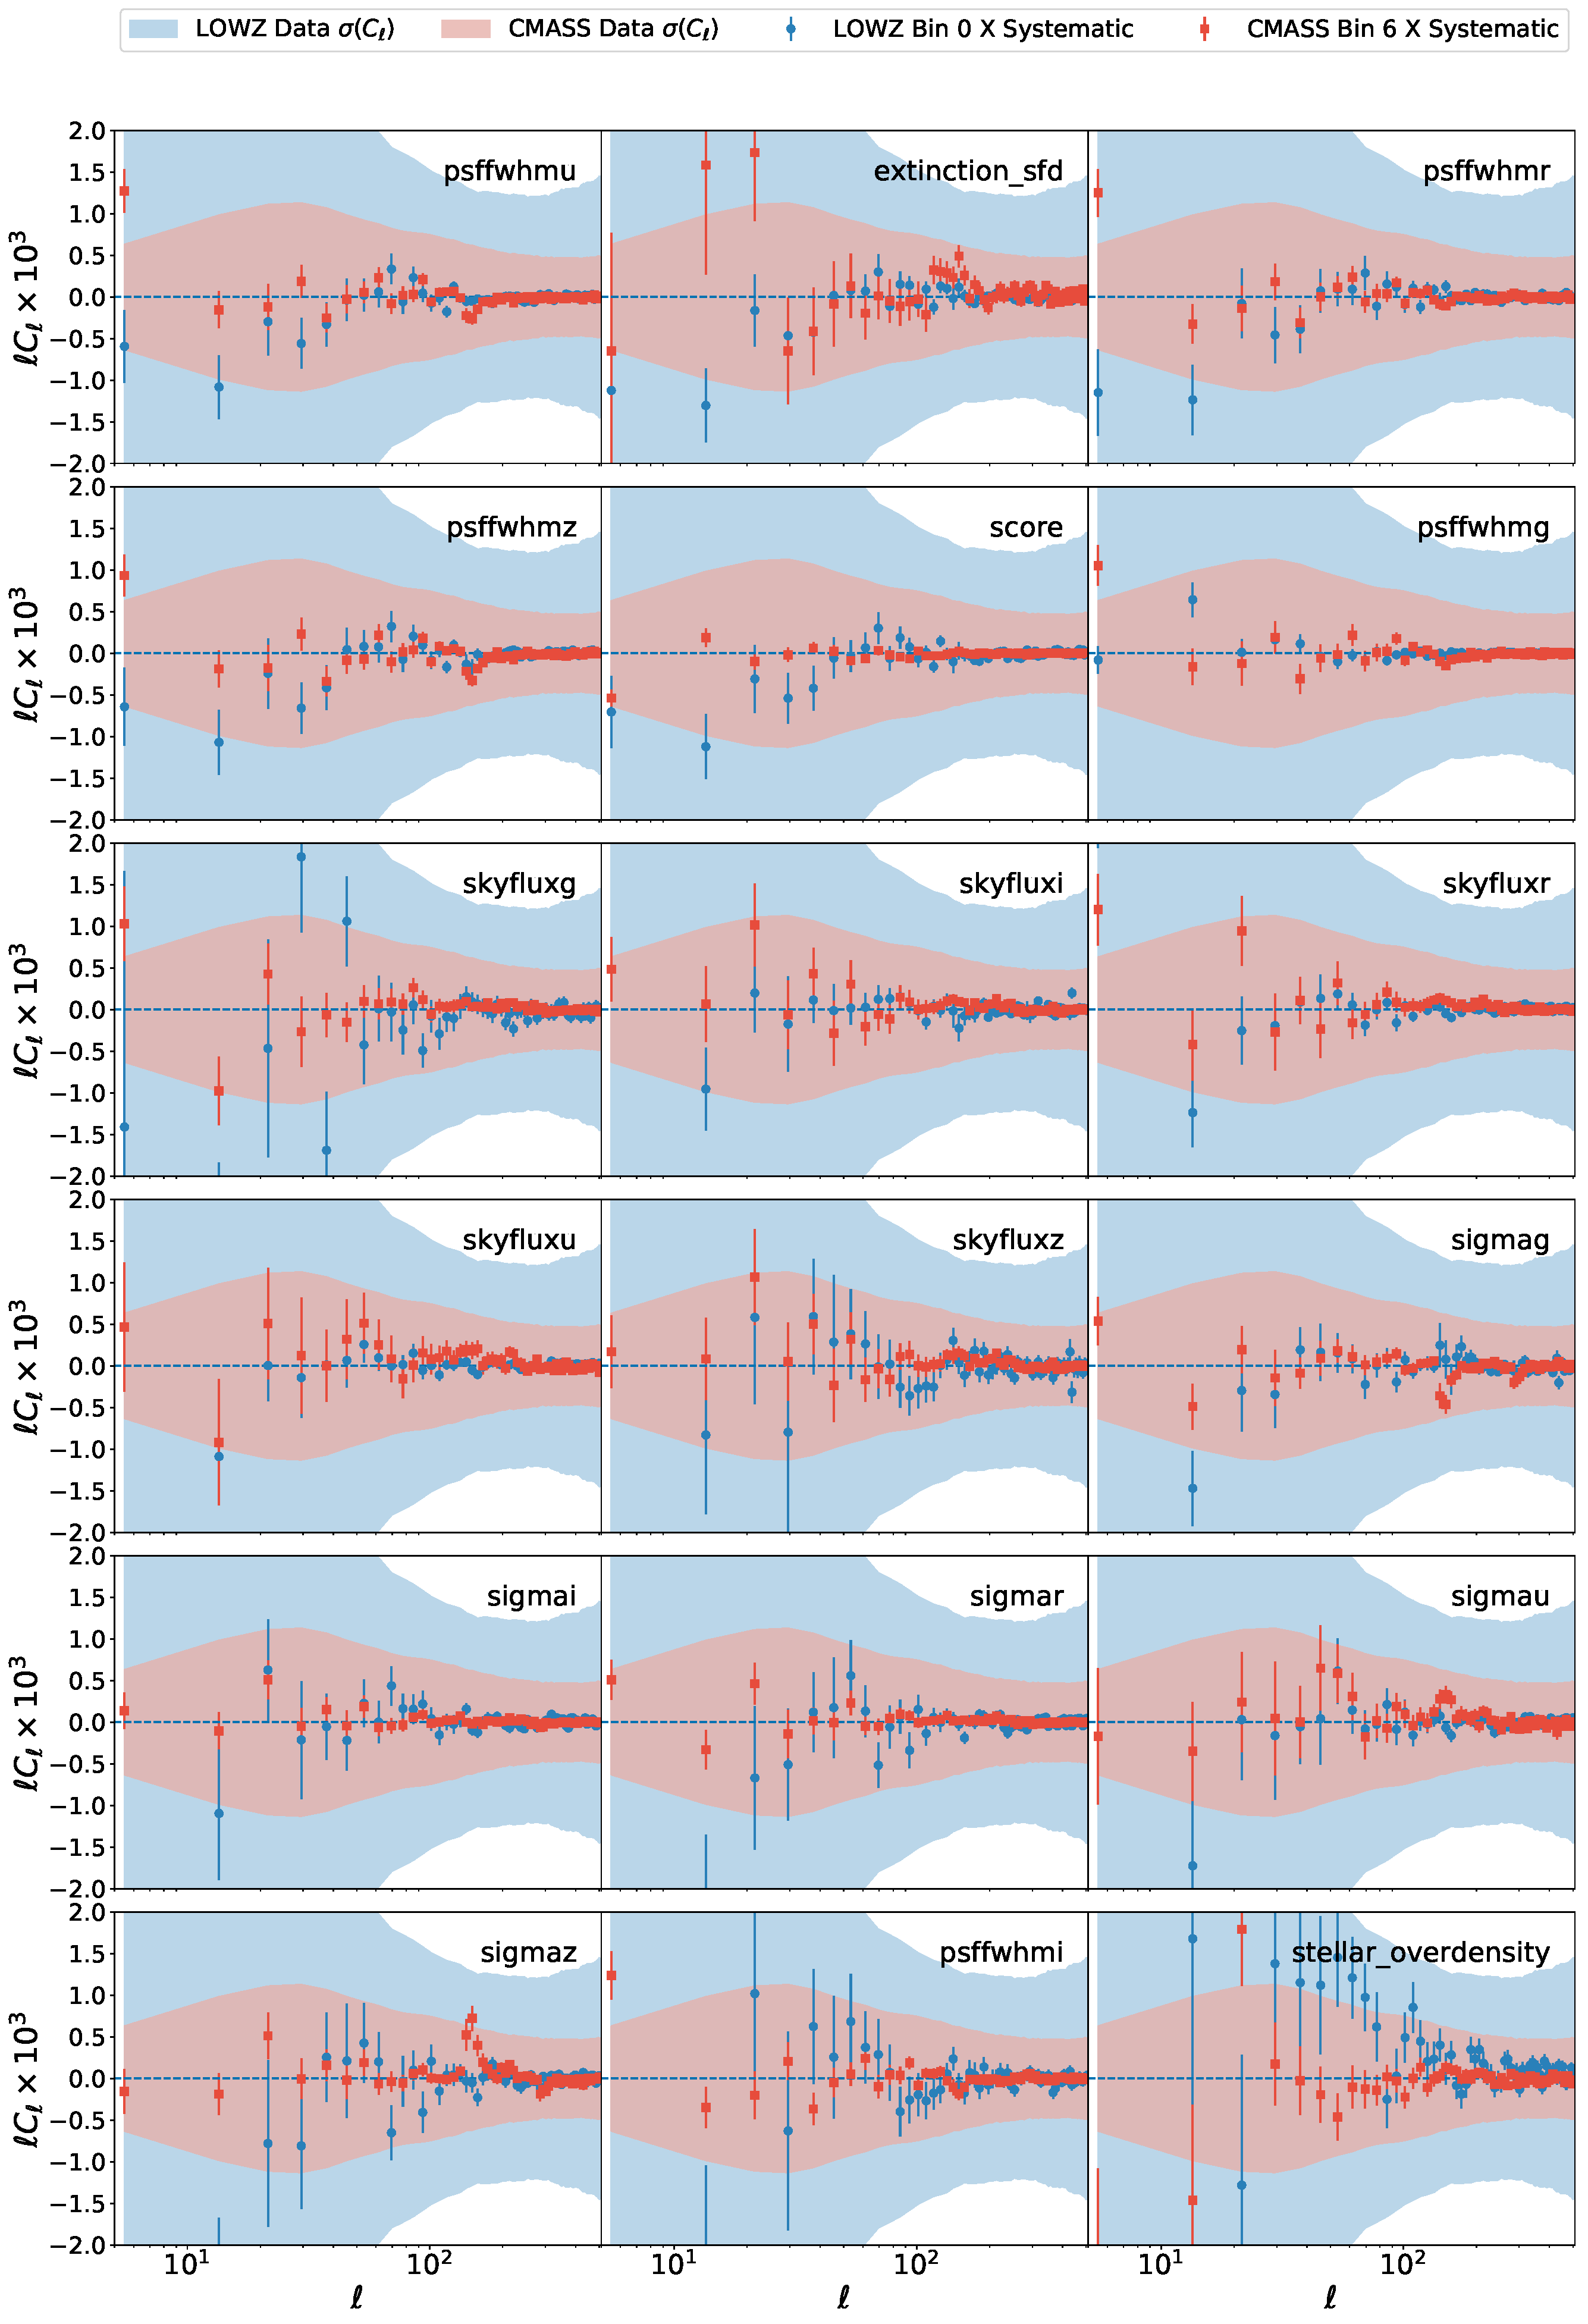
\includegraphics[width=\textwidth]{BOSS-FIGS/systematics_CMASS_Bin0_LOWZ_Bin0.pdf}
\caption[Cross-power spectra between systematics and LOWZ--0(CMASS--6) tomographic bins.]{Cross-power spectra between the 18 systematics overdensity maps produced in \ref{Sec:SystMaps}, and LOWZ--0(CMASS--6) tomographic bins in blue dots (red squares). The error-bars were obtained by cross-correlating the $\delta^{Sys}$ maps with the \texttt{FLASK} mocks produced in Section \ref{Sec:Cov}; the shaded region shows the variance of the data, which was also obtained from the same mocks.}
\label{fig:SystBin0}
\end{center}
\end{figure*}

\begin{figure*}
\begin{center}
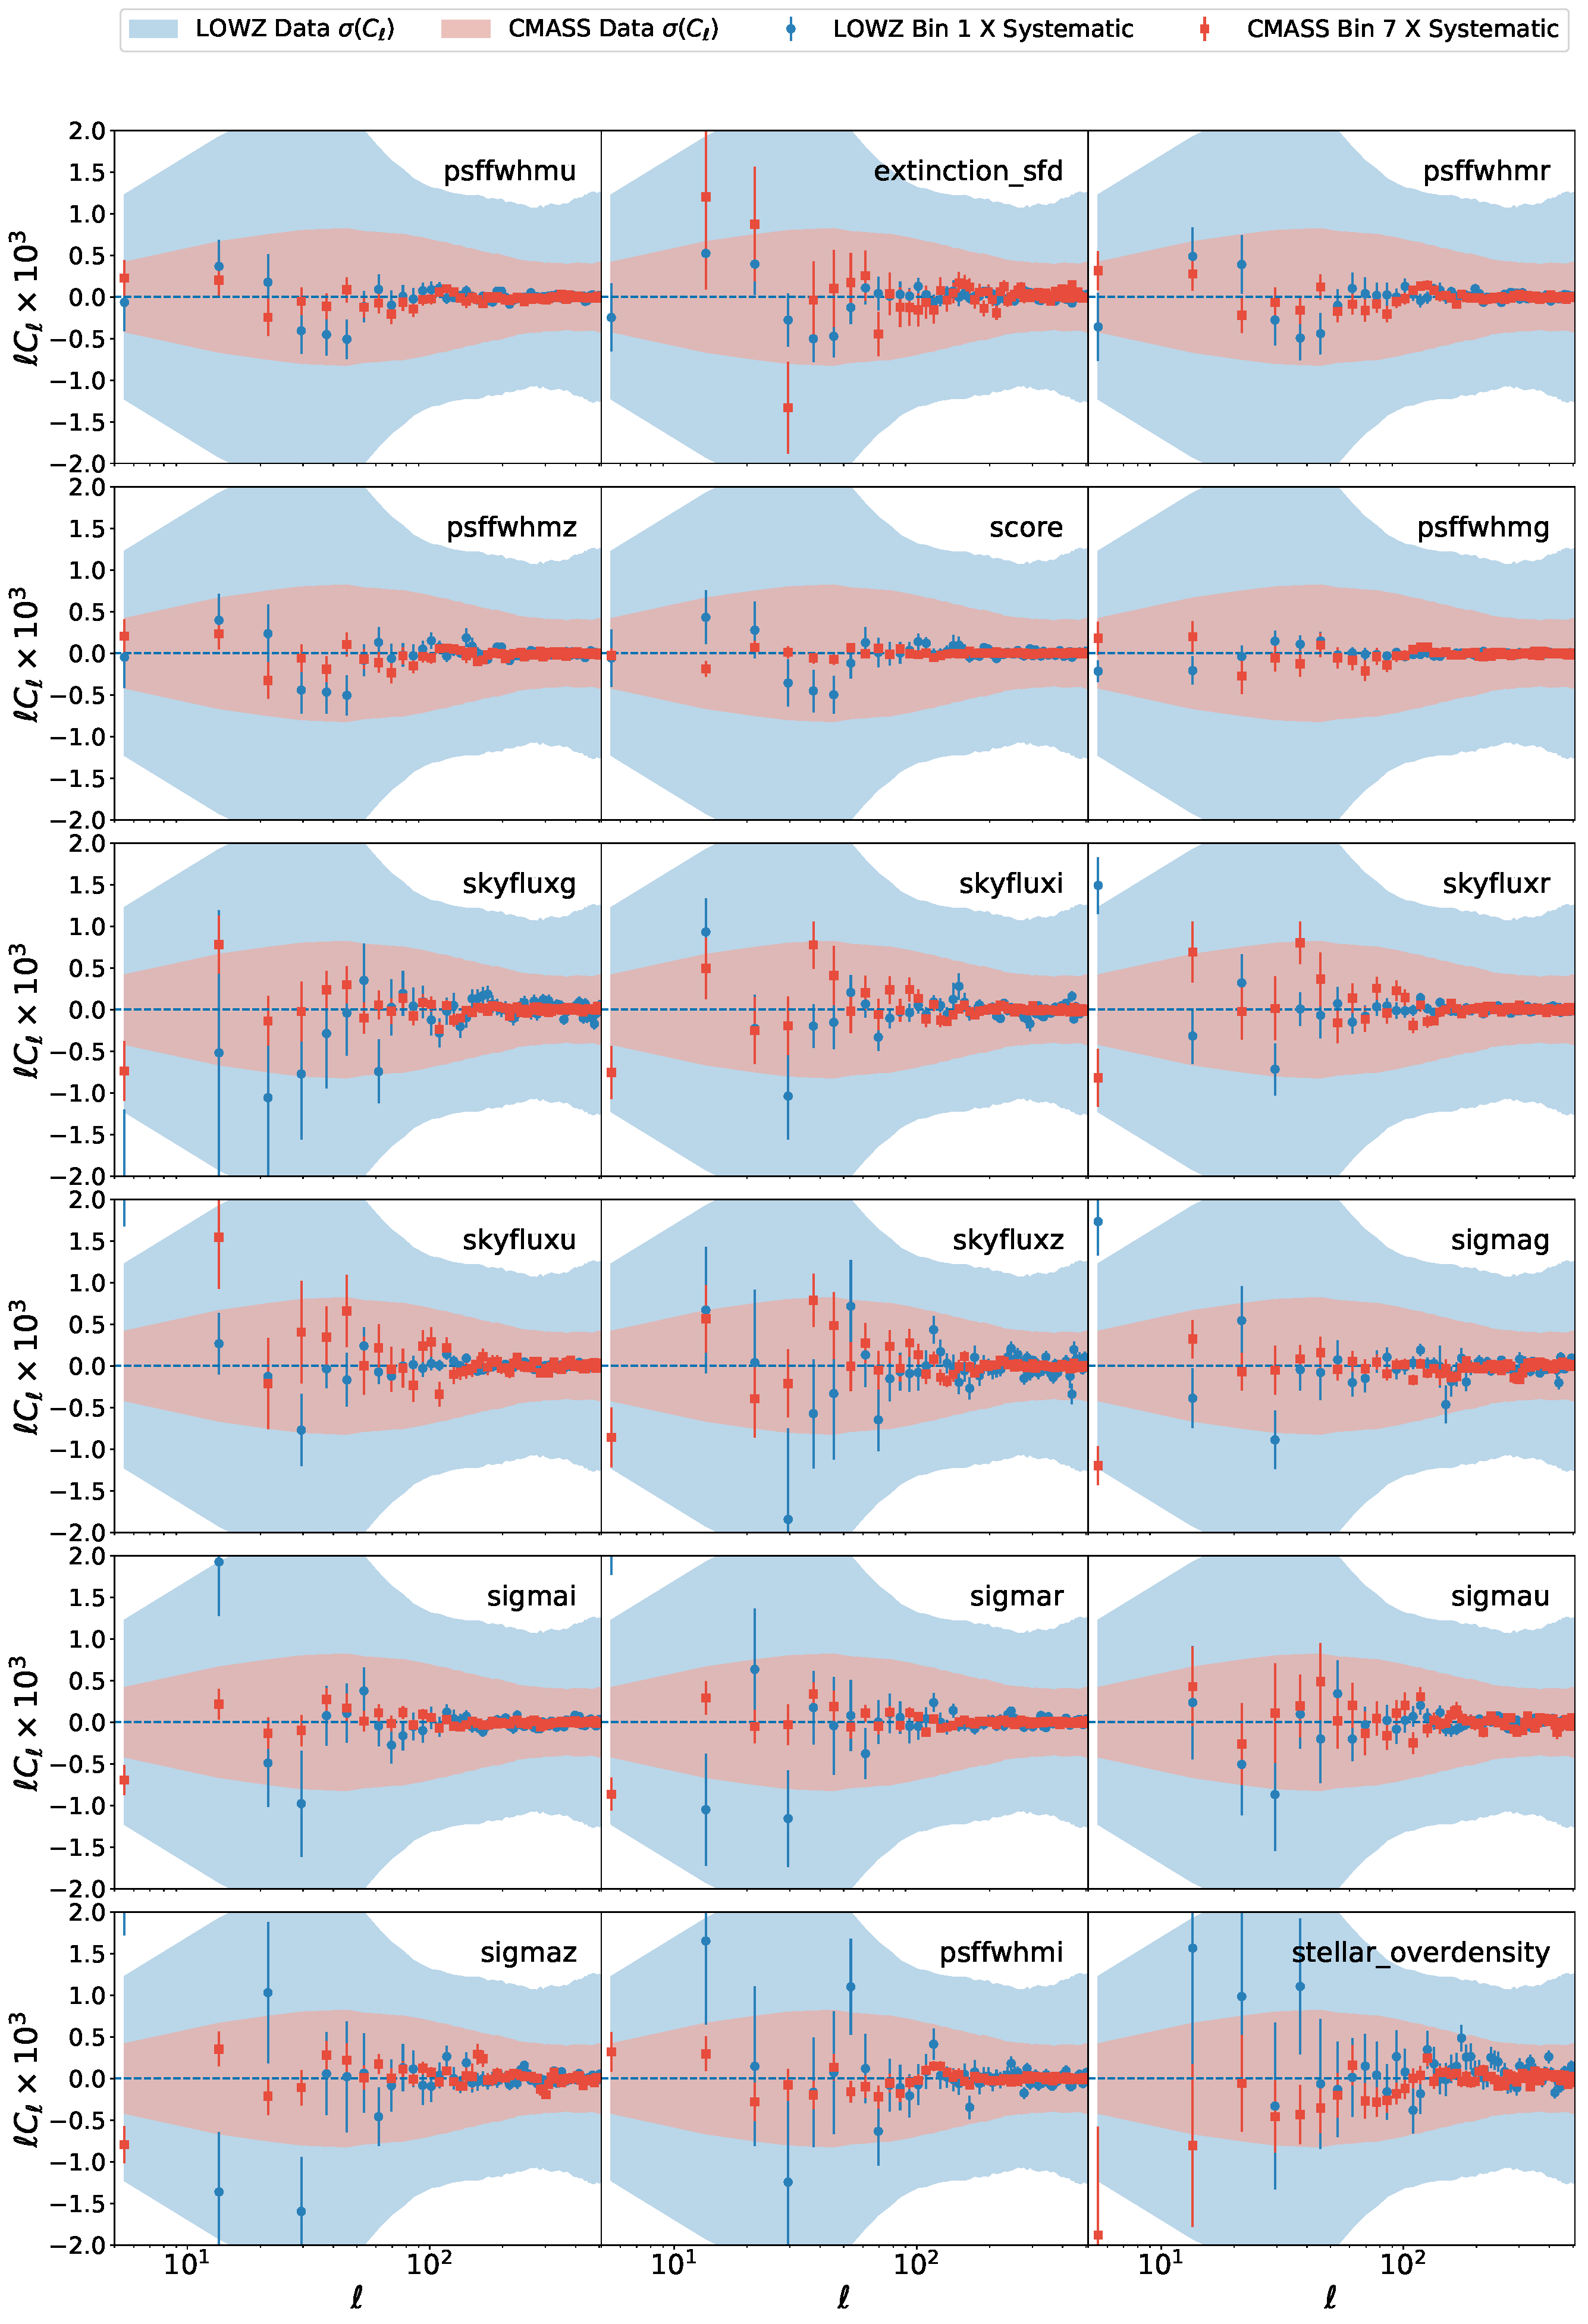
\includegraphics[width=\textwidth]{BOSS-FIGS/systematics_CMASS_Bin1_LOWZ_Bin1.pdf}
\caption[Cross-power spectra between systematics and LOWZ--1(CMASS--7) tomographic bins.]{Cross-power spectra between the 18 systematics overdensity maps produced in \ref{Sec:SystMaps}, and LOWZ--1(CMASS--7) tomographic bins in blue dots (red squares). The error-bars were obtained by cross-correlating the $\delta^{Sys}$ maps with the \texttt{FLASK} mocks produced in Section \ref{Sec:Cov}; the shaded region shows the variance of the data, which was also obtained from the same mocks.}
\label{fig:SystBin1}
\end{center}
\end{figure*}

\begin{figure*}
\begin{center}
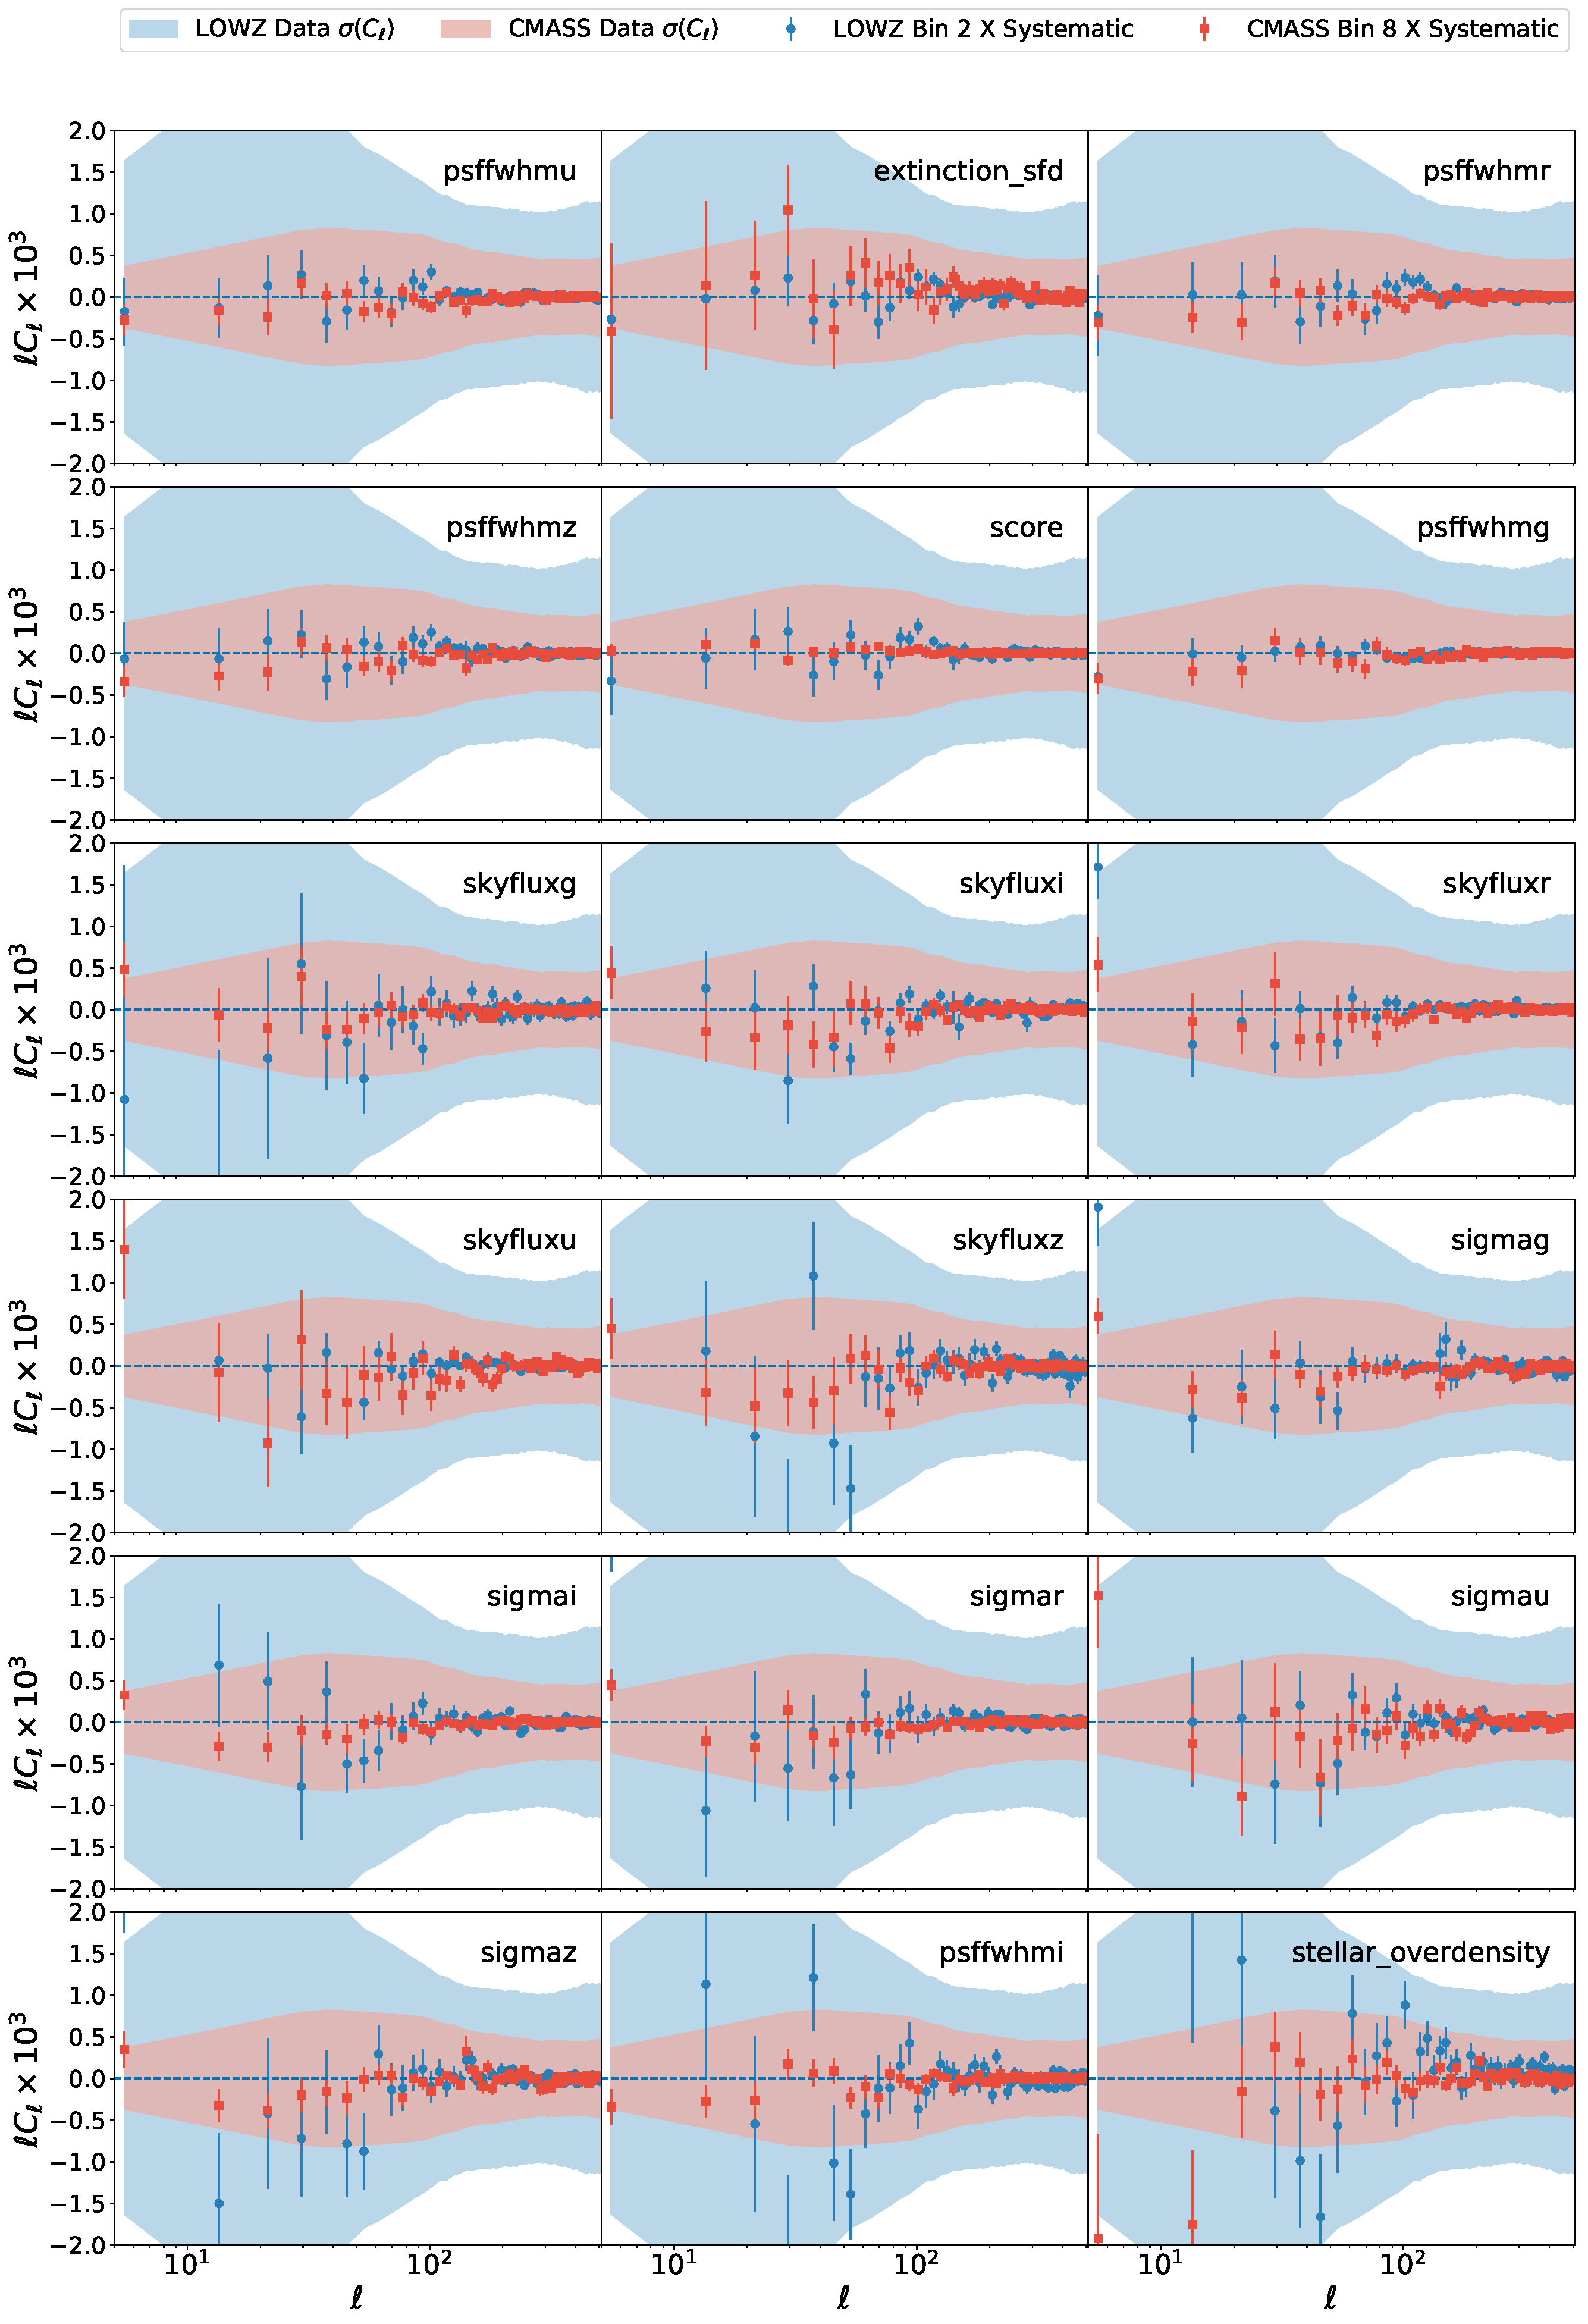
\includegraphics[width=\textwidth]{BOSS-FIGS/systematics_CMASS_Bin2_LOWZ_Bin2.pdf}
\caption[Cross-power spectra between systematics and LOWZ--2(CMASS--8) tomographic bins.]{Cross-power spectra between the 18 systematics overdensity maps produced in \ref{Sec:SystMaps}, and LOWZ--2(CMASS--8) tomographic bins in blue dots (red squares). The error-bars were obtained by cross-correlating the $\delta^{Sys}$ maps with the \texttt{FLASK} mocks produced in Section \ref{Sec:Cov}; the shaded region shows the variance of the data, which was also obtained from the same mocks.}
\label{fig:SystBin2}
\end{center}
\end{figure*}

\begin{figure*}
\begin{center}
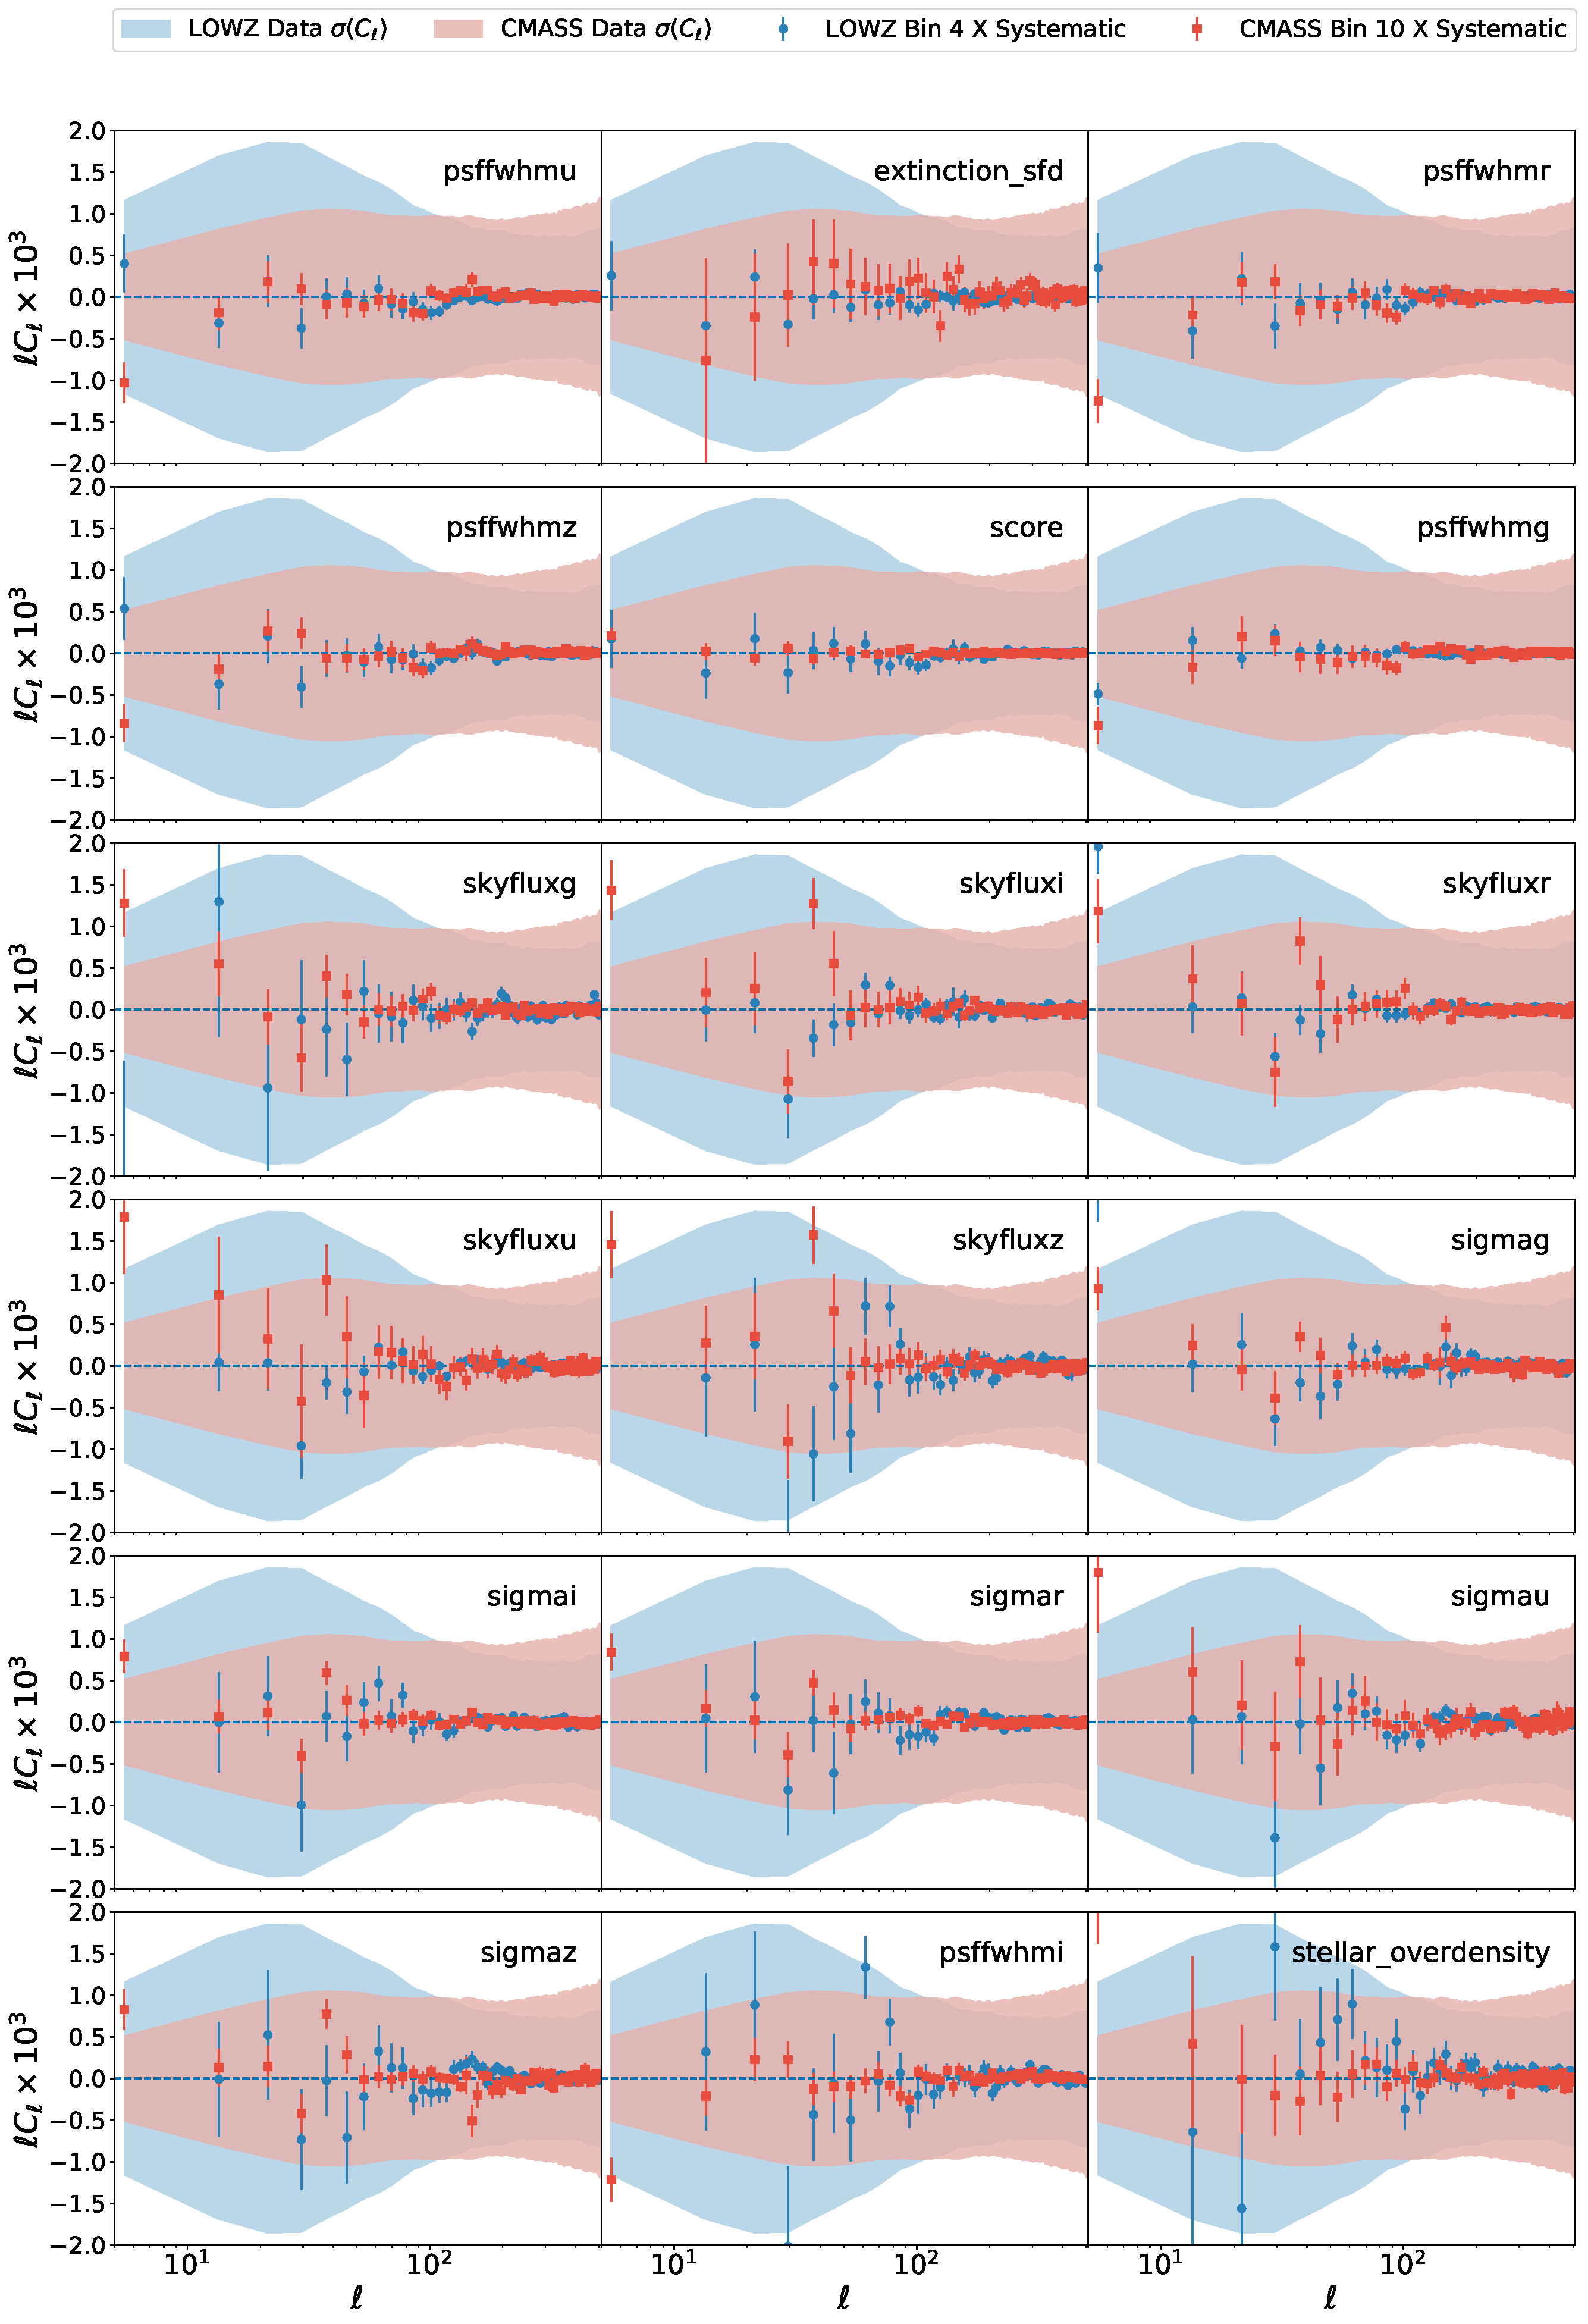
\includegraphics[width=\textwidth]{BOSS-FIGS/systematics_CMASS_Bin4_LOWZ_Bin4.pdf}
\caption[Cross-power spectra between systematics and LOWZ--4(CMASS--10) tomographic bins.]{Cross-power spectra between the 18 systematics overdensity maps produced in \ref{Sec:SystMaps}, and LOWZ--4(CMASS--10) tomographic bins in blue dots (red squares). The error-bars were obtained by cross-correlating the $\delta^{Sys}$ maps with the \texttt{FLASK} mocks produced in Section \ref{Sec:Cov}; the shaded region shows the variance of the data, which was also obtained from the same mocks.}
\label{fig:SystBin4}
\end{center}
\end{figure*}

\begin{figure*}
\begin{center}
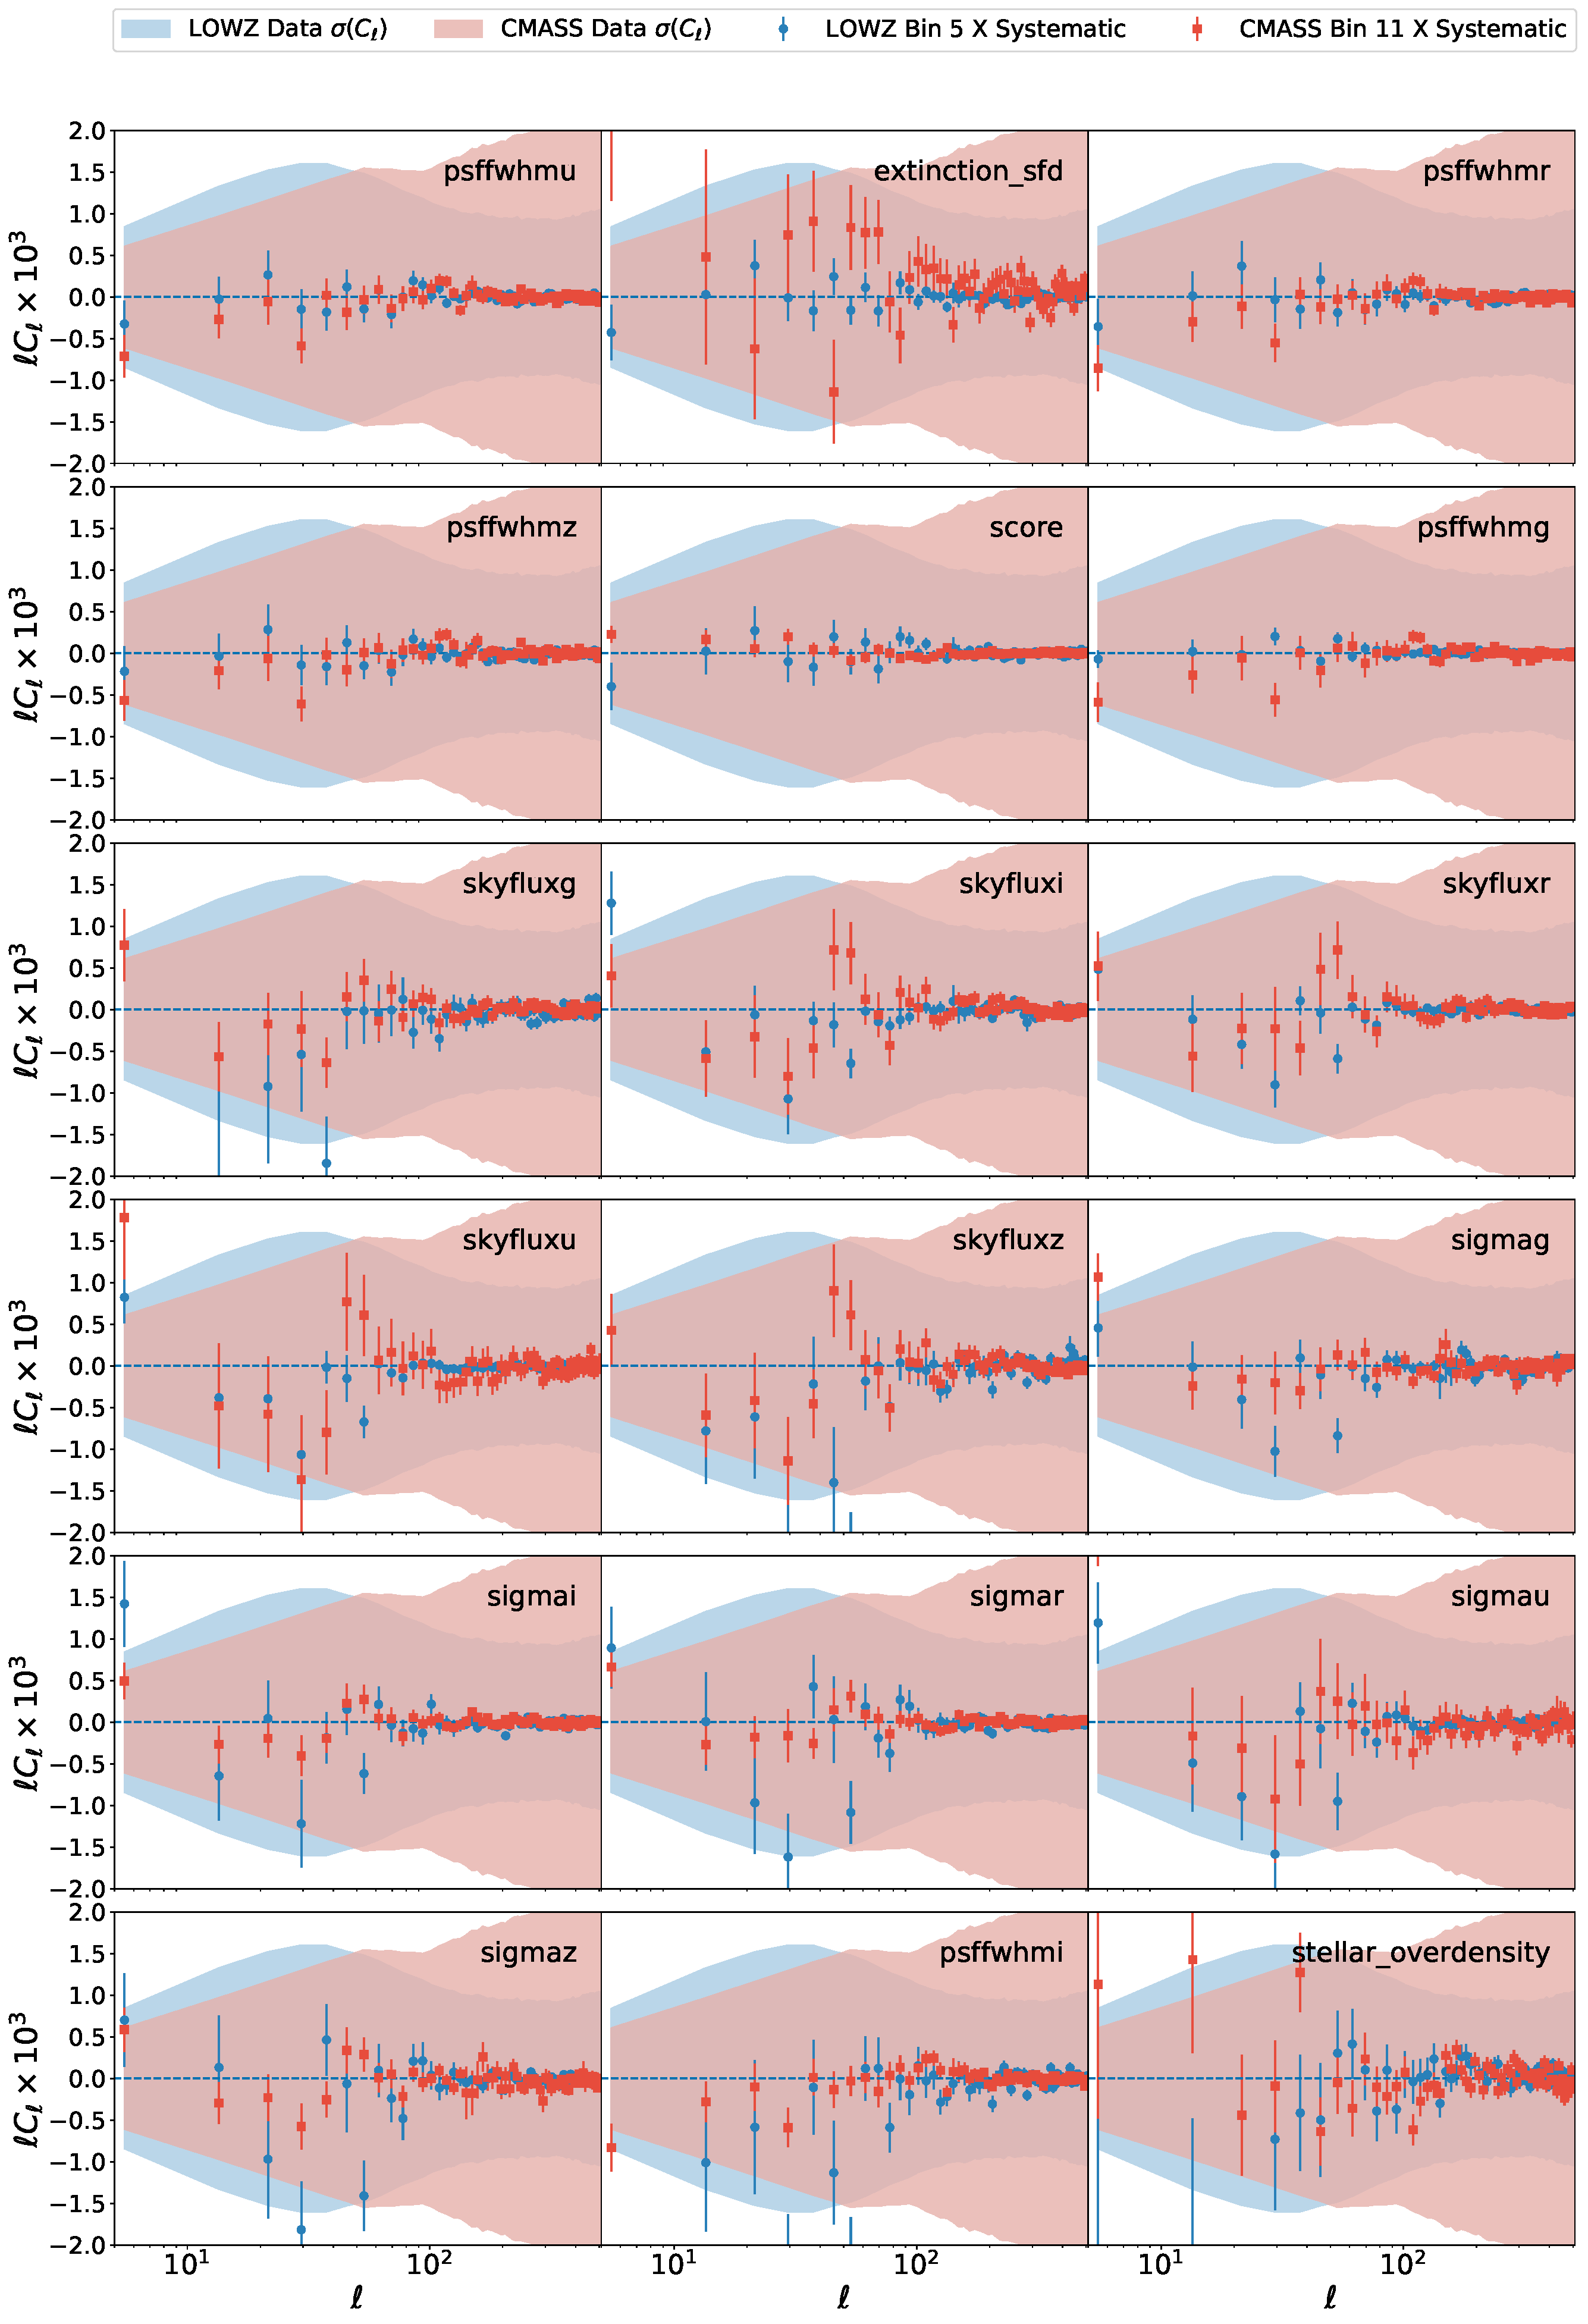
\includegraphics[width=\textwidth]{BOSS-FIGS/systematics_CMASS_Bin5_LOWZ_Bin5.pdf}
\caption[Cross-power spectra between systematics and LOWZ--5(CMASS--11) tomographic bins.]{Cross-power spectra between the 18 systematics overdensity maps produced in \ref{Sec:SystMaps}, and LOWZ--5(CMASS--11) tomographic bins in blue dots (red squares). The error-bars were obtained by cross-correlating the $\delta^{Sys}$ maps with the \texttt{FLASK} mocks produced in Section \ref{Sec:Cov}; the shaded region shows the variance of the data, which was also obtained from the same mocks.}
\label{fig:SystBin5}
\end{center}
\end{figure*}

\begin{figure*}
\begin{center}
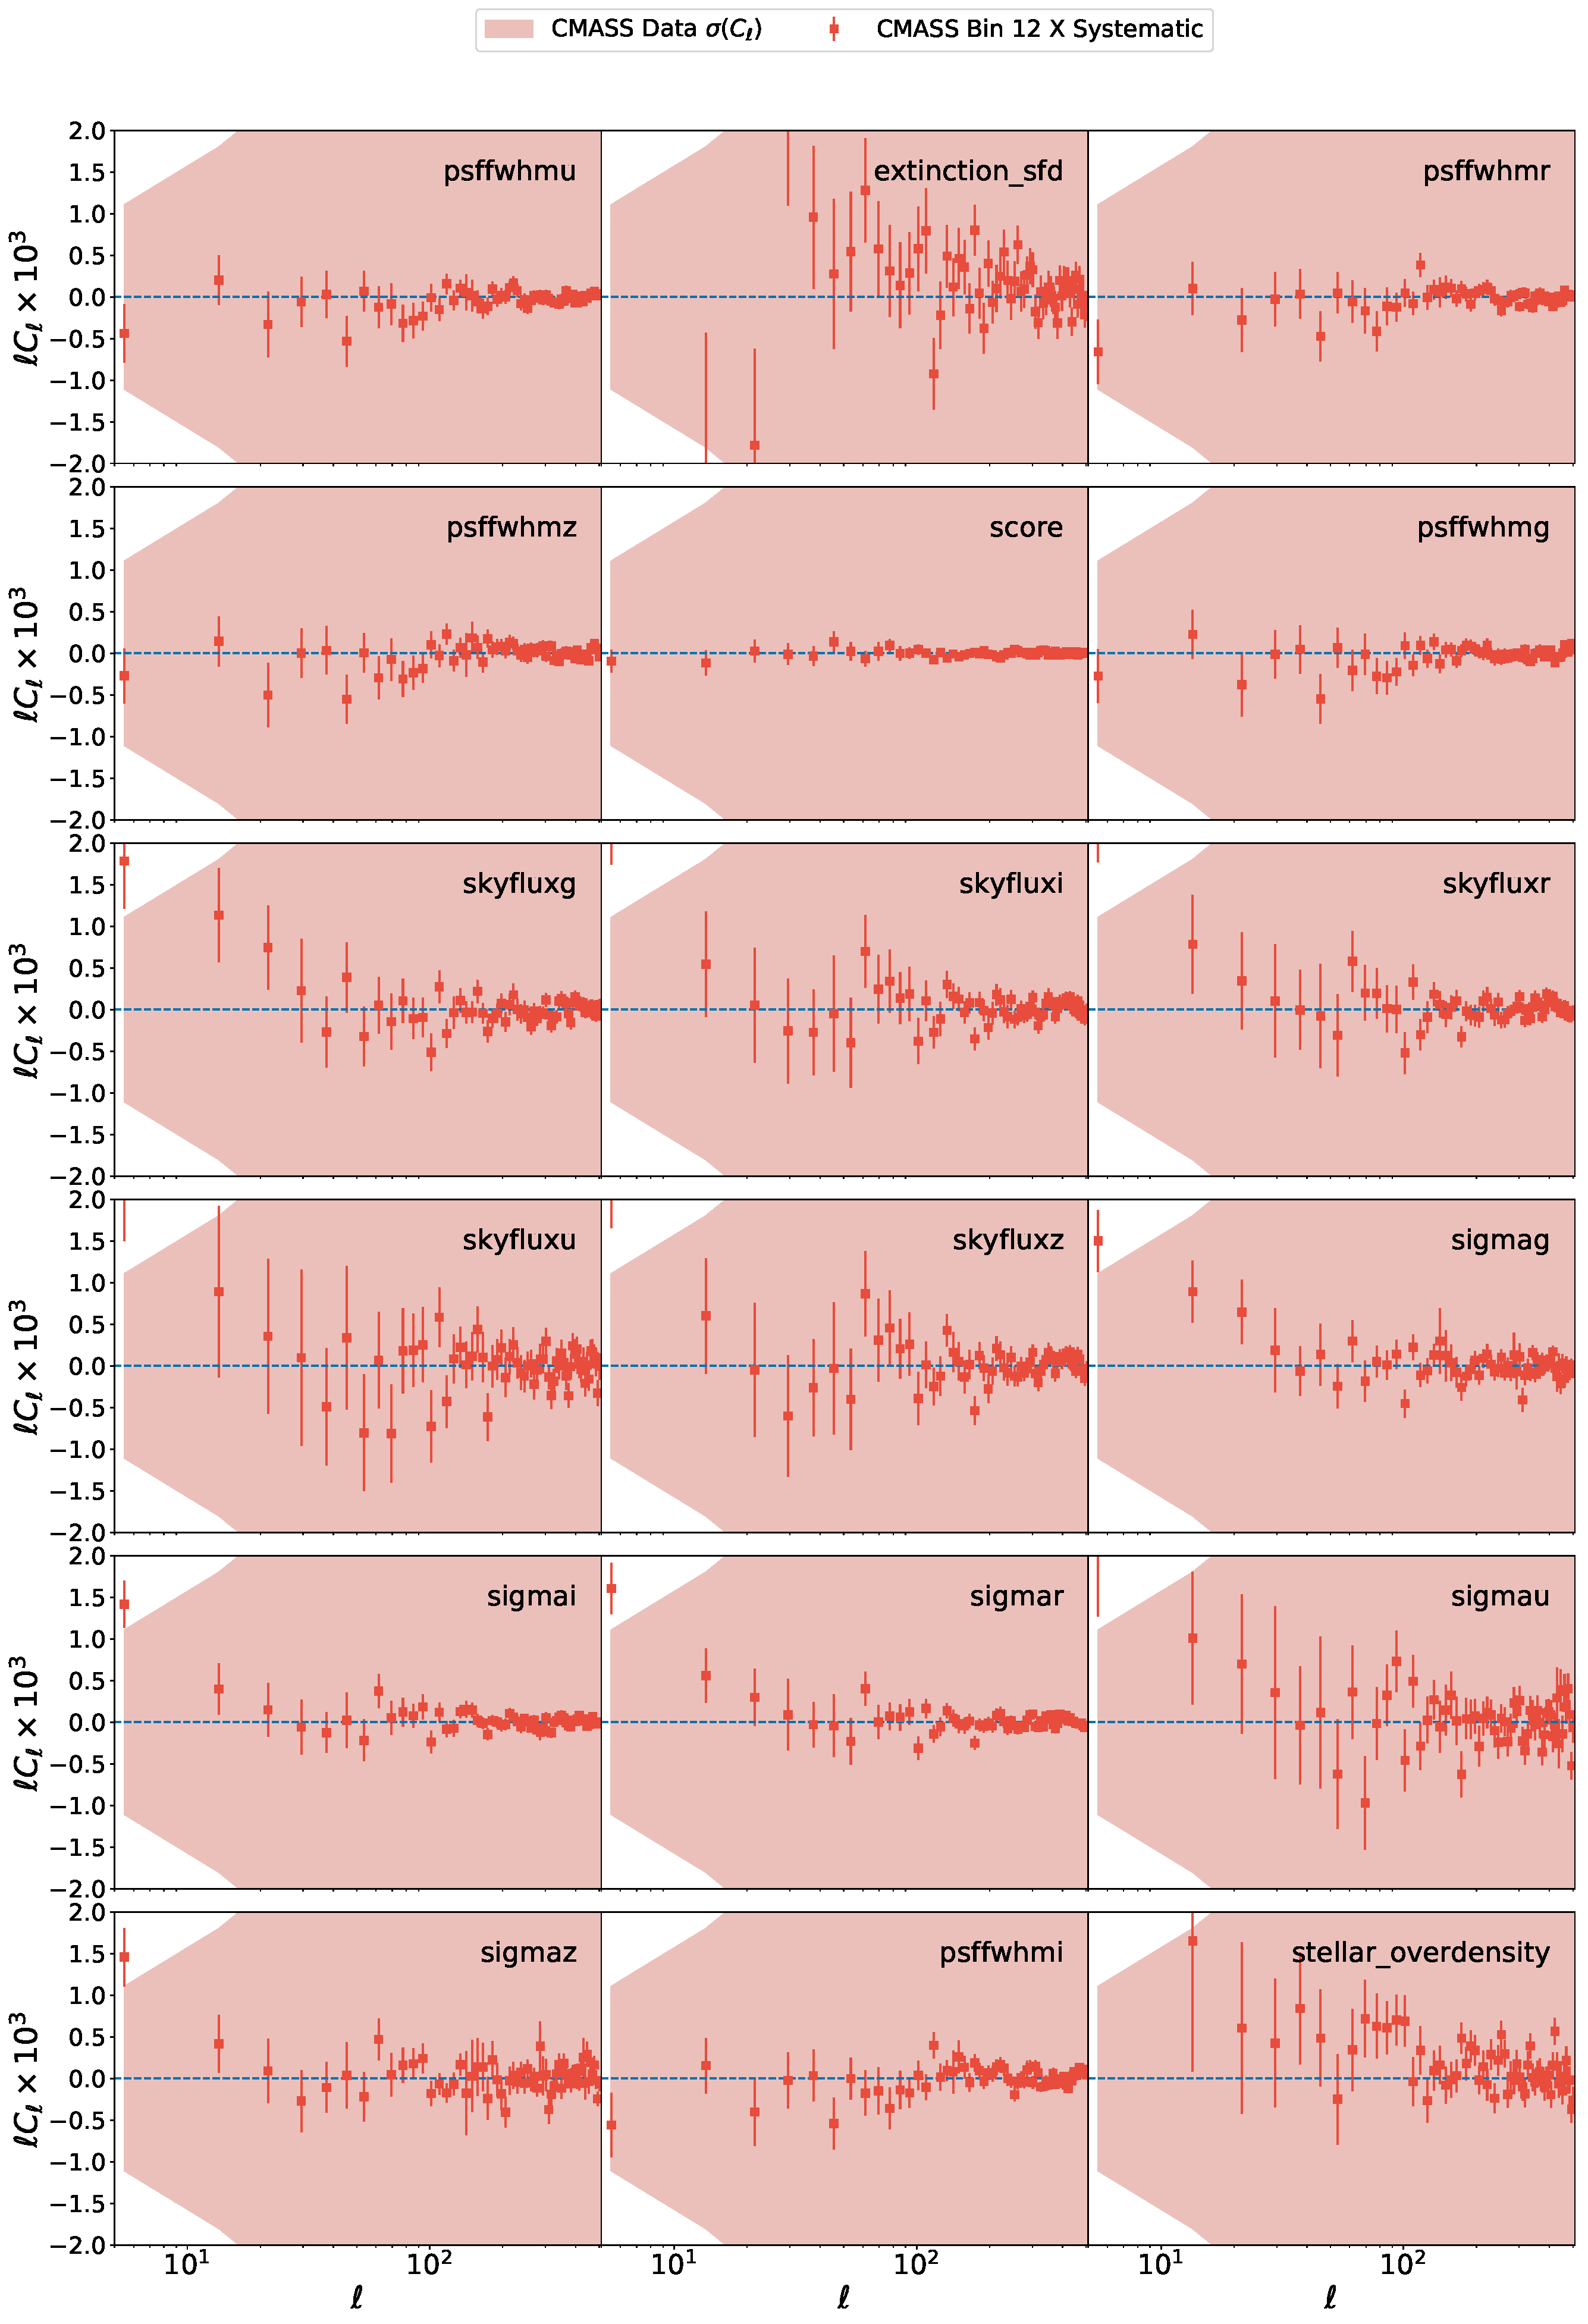
\includegraphics[width=\textwidth]{BOSS-FIGS/systematics_CMASS_Bin6_LOWZ_Bin6.pdf}
\caption[Cross-power spectra between systematics and CMASS--12 tomographic bins. ]{Cross-power spectra between the 18 systematics overdensity maps produced in \ref{Sec:SystMaps} CMASS--12 tomographic bin in red squares. The error-bars were obtained by cross-correlating the $\delta^{Sys}$ maps with the \texttt{FLASK} mocks produced in Section \ref{Sec:Cov}; the shaded region shows the variance of the data, which was also obtained from the same mocks.}
\label{fig:SystBin6}
\end{center}
\end{figure*}





